%%%%%%%%%%%%%%%%%%%%%%%%%%%%%%%%%%%%%%%%%%%%%%%%%%%%%%%%%%%%%%%%%%%%%%%%%%%%%%
%%  Safe designs, unsafe ecosystems: deployment-layer selection in an
%%  evolutionary AI race
%%
%%  Prepared for: Autonomous Agents and Multi-Agent Systems (JAAMAS), Springer
%%  Template:     Springer Nature sn-jnl.cls, v3.1 (December 2024)
%%
%%  Build:  pdflatex main && bibtex main && pdflatex main && pdflatex main
%%          (or: python build.py)
%%
%%  This file is generated from ../paper/main.tex by ../scripts/build_jaamas.py.
%%  Edit the generator, not this file, unless you are finalising the submission.
%%%%%%%%%%%%%%%%%%%%%%%%%%%%%%%%%%%%%%%%%%%%%%%%%%%%%%%%%%%%%%%%%%%%%%%%%%%%%%
\documentclass[pdflatex]{sn-jnl}

%%============================================================================%%
%%  Reference style
%%
%%  JAAMAS cites by number in square brackets and prints an APA-formatted
%%  reference list.  The Springer class ties citation form and list form
%%  together (sn-apa gives author-year citations, sn-basic gives non-APA
%%  entries), so neither option alone matches the journal.  We therefore load
%%  Springer's own APA machinery and switch natbib into numeric mode by hand,
%%  and use sn-apanum.bst, which is Springer's sn-apacite.bst with its sorting
%%  passes suppressed so the list comes out in citation order.
%%============================================================================%%
\usepackage[natbibapa]{apacite}
\makeatletter
\providecommand{\BPBI}{.}%                      period between initials
\setlength{\bibsep}{1em}%
\def\bibfont{\reset@font\fontfamily{\rmdefault}\normalsize\selectfont}%
\def\refdoi#1{\urlstyle{rm}\url{#1}}%
\providecommand{\doiprefix}{}\renewcommand{\doiprefix}{}%
\gdef\NumBib{YES}%
\setcitestyle{numbers,square,comma,sort&compress}
\def\@biblabel#1{[#1]}
\renewenvironment{thebibliography}[1]{%
  \section*{\refname}%
  \bibfont
  \list{\@biblabel{\@arabic\c@enumiv}}%
       {\settowidth\labelwidth{\@biblabel{#1}}%
        \leftmargin\labelwidth \advance\leftmargin\labelsep
        \setlength{\itemsep}{\bibsep}\setlength{\parsep}{\z@}%
        \usecounter{enumiv}\let\p@enumiv\@empty
        \renewcommand\theenumiv{\@arabic\c@enumiv}}%
  \let\newblock\relax
  \sloppy\clubpenalty4000\@clubpenalty\clubpenalty\widowpenalty4000%
  \sfcode`\.\@m}
 {\def\@noitemerr{\@latex@warning{Empty `thebibliography' environment}}%
  \endlist}
\makeatother
\bibliographystyle{sn-apanum}

%%============================================================================%%
%%  Packages.  sn-jnl already provides geometry, fontenc, hyperref, amsthm,
%%  appendix, rotating, threeparttable and wrapfig, so none of those is
%%  reloaded here.
%%============================================================================%%
\usepackage{graphicx}
%%  The figures sit in figures/ in the submission package, but Editorial
%%  Manager unpacks every uploaded file into one flat directory, so ./ is
%%  searched too and the same source compiles under either layout.
\graphicspath{{figures/}{./}}
\usepackage{amsmath,amssymb,amsfonts}
\usepackage{booktabs}
\usepackage{multirow}
\usepackage{microtype}
\usepackage{xcolor}

%%============================================================================%%
%%  Theorem environments
%%============================================================================%%
\theoremstyle{thmstyleone}
\newtheorem{theorem}{Theorem}
\newtheorem{proposition}[theorem]{Proposition}
\newtheorem{lemma}[theorem]{Lemma}
\newtheorem{corollary}[theorem]{Corollary}
\theoremstyle{thmstylethree}
\newtheorem{definition}[theorem]{Definition}
\theoremstyle{thmstyletwo}
\newtheorem{remark}{Remark}

%%============================================================================%%
%%  Notation carried over from the source manuscript
%%============================================================================%%
\definecolor{cAS}{HTML}{0072B2}
\definecolor{cAU}{HTML}{D55E00}
\definecolor{cCS}{HTML}{009E73}
\definecolor{cCAS}{HTML}{CC79A7}

\newcommand{\AS}{\textsf{AS}}
\newcommand{\AU}{\textsf{AU}}
\newcommand{\CS}{\textsf{CS}}
\newcommand{\CAS}{\textsf{CAS}}
\newcommand{\piP}{\pi_{P}}
\newcommand{\piS}{\pi_{S}}
\newcommand{\R}{\mathbb{R}}
\newcommand{\Simplex}{\Delta_{n}}

\begin{document}

%%============================================================================%%
%%  Title page
%%
%%  All three authors contributed equally: the shared first authorship is
%%  carried by \equalcont, which sets a dagger on each name.  ORCIDs are
%%  supplied through the Editorial Manager submission form, which is where
%%  Springer collects them.  Springer will not accept changes to the author
%%  list after acceptance.
%%============================================================================%%
\title[Deployment-layer selection in an evolutionary AI race]{Safe designs,
unsafe ecosystems: deployment-layer selection in an evolutionary AI race}

\author*[1,2]{\fnm{Trung-Kiet} \sur{Huynh}}\email{23122039@student.hcmus.edu.vn}
\equalcont{These authors contributed equally to this work.}

\author[1,2]{\sur{Dao Sy Duy} \fnm{Minh}}\email{23122041@student.hcmus.edu.vn}
\equalcont{These authors contributed equally to this work.}

\author[1,2]{\fnm{Chi-Nguyen} \sur{Tran}}\email{23122044@student.hcmus.edu.vn}
\equalcont{These authors contributed equally to this work.}

\affil*[1]{\orgdiv{Faculty of Information Technology},
\orgname{University of Science (HCMUS)},
\orgaddress{\city{Ho Chi Minh City}, \country{Vietnam}}}

\affil[2]{\orgname{Vietnam National University -- Ho Chi Minh City (VNU-HCM)},
\orgaddress{\city{Ho Chi Minh City}, \country{Vietnam}}}

%%  JAAMAS asks for 150 to 250 words, no citations, no equations, no undefined
%%  abbreviations, and 4 to 6 keywords.  build.py counts both.
\abstract{An ecosystem of deployed autonomous agents is selected twice over. An
agent earns a payoff by acting for a principal, but whether its design spreads
is decided by that principal, who never plays the game and bears only part of
the harm it causes. Evolutionary game theory normally identifies the two. We
call their difference the selection wedge, embed it in a four-strategy model of
an artificial intelligence race, and analyse its replicator and
finite-population dynamics. The wedge collapses to a single control parameter,
an effective liability, in which every invasion condition is affine, so all
thresholds are closed form. Four consequences follow for governance. Screening
designs before deployment, at any tolerance that admits reciprocation, removes
only a weakly dominated design and leaves the long-run unsafe frequency
unchanged. That frequency is not monotone in liability: over an intermediate
window liability also taxes the retaliation on which conditional safety
depends, the unsafe state becomes uninvadable by conditional safety, and
crossing the window's lower edge from below lifts the basin-weighted unsafe
frequency from zero to about a third. The barrier protecting a safe population
meanwhile varies by a factor of 77.7, at the baseline calibration, along a
composition that selection leaves neutral. And irreversible capability
diffusion makes the loss of a protected regime hysteretic, with exactly
computable width. Governance of such an ecosystem binds at the layer that
selects designs, not at the layer that plays them.}

\keywords{Multi-agent systems, Evolutionary game theory, Replicator dynamics,
Liability, Artificial intelligence governance}

\maketitle

\section{Introduction}

Evolutionary game theory usually identifies two things that need not be the
same: the payoff an individual earns in the game, and the quantity that
governs how often that individual is copied~\citep{maynardsmith1982evolution,taylor1978evolutionarily,hofbauer1998evolutionary,hofbauer2003evolutionary,nowak2006evolutionary}.
Under that identification every standard result -- the correspondence between
rest points and Nash equilibria, the stability of evolutionarily stable
strategies, the invasion analysis of finite populations -- is a statement
about one payoff matrix used twice.

Ecosystems of deployed AI agents break the identification in a specific way.
An agent negotiates, bids, schedules or races on behalf of a principal, and
earns a payoff by doing so. Such populations already exist in narrow form:
autonomous pricing algorithms deployed by competing sellers converge on
supra-competitive outcomes without any communication or intent to
collude~\citep{calvano2020collusion}, and when many deployers select from the
same small pool of designs the resulting correlation is itself a source of
social loss~\citep{kleinberg2021monoculture}. In both cases the object that
propagates is a design chosen by a deployer, not a behaviour chosen by the
system that plays. Populations of interacting language-model agents likewise
develop collective properties that no single agent carries -- emergent
conventions and collective bias~\citep{ashery2025emergent}, and cooperation
levels shaped by transmission across generations of
agents~\citep{vallinder2024cultural,willis2025llm}. Whether the agent's \emph{design} -- its model,
its system prompt, its scaffold -- is replicated across further deployments
is not decided by the agent, and is not decided by the payoff the agent earned
in the abstract. It is decided by the principal who deployed it, on the basis
of what the principal received. The two quantities differ whenever the design
imposes costs on third parties that the principal does not bear. The
replicating unit is therefore selected by an agent that never plays the game,
according to a functional that is not the social one. Selection here is
artificial rather than natural, in the breeder's sense: the copied variant is
the one that served the breeder.

That makes this a multi-agent systems problem rather than a modelling
curiosity. A deployed agent ecosystem is a multi-agent system whose
composition is chosen by nobody inside it: an agent's autonomy does not move
responsibility for its conduct away from the humans who deploy
it~\citep{chan2023harms}, whose ethical and legal boundaries are still being
drawn as agents take initiative at wider levels~\citep{wellman2017ethical},
and who bear part of the harm it causes and all of the decision about whether
that design is deployed again. The instruments this field has built for open
agent populations act from within the interaction. Social laws restrict the
strategies an agent may use~\citep{shoham1995social}, electronic institutions
enforce the protocols it must follow~\citep{arcos2005electronic}, norms spread
and are sanctioned among the agents that carry
them~\citep{morrismartin2019norm,nardin2016sanctions}, reputation aggregates
past behaviour into a signal its partners condition
on~\citep{huynh2006integrated}, and reward transfers and formal contracts
alter the payoffs it faces~\citep{willis2024minimal,haupt2024contracts}. The
design-selection channel fixes the membership of the population all of them
act on, through an actor none of them prices and on a functional none of them
makes an object of policy.

The consequences of that decoupling are the subject of this paper. They are
not the familiar observation that individual incentives can diverge from
collective welfare, which has been understood since Hardin's account of the
commons~\citep{hardin1968tragedy,ostrom1990governing} and is the content of
every social dilemma.
The point is structural and sharper: the dynamical system that describes the
deployed population is the replicator equation of a game that nobody plays.
Its rest points are the equilibria of the principals' selection game, and the
social game enters only as a passive observable. Interventions therefore have
very different effects depending on which of the two objects they touch. An
intervention on the design pool -- safety training, capability evaluations,
release gating, which is where most current frontier-AI regulation
sits~\citep{anderljung2023frontier,euaiact2024} -- changes the set of
available strategies. An intervention on the selection functional --
liability, disclosure, procurement rules -- changes the vector field itself.
We show that the first class can be exactly
neutral while the second class is not, and that the second class can be
non-monotone in a way that makes an intermediate range of it worse than a
weaker setting.

The separation itself is not new. The indirect evolutionary approach~\citep{guth1992evolutionary,guth1995evolutionary,dekel2007evolution,alger2013homo},
surveyed by~\citet{alger2019preference},
studies populations in which behaviour follows subjective preferences while
selection operates on material payoffs, and~\citet{heifetz2007maximize} show
that in almost every game some distortion of a player's true payoff is
beneficial and survives payoff-monotone selection. Our construction is the
mirror image. There the distortion sits in the behaviour and is selected on
the socially correct functional, and it is endogenous; here behaviour follows
the material race payoff, the distortion sits in the \emph{selection}
functional, and it is an exogenous policy parameter. What is new is not the
existence of two functionals but the direction of the wedge and its
consequences for governance instruments, which is why our results are
statements about interventions rather than about which preferences survive.

Concern about selection pressure over deployed AI systems has been raised
informally~\citep{hendrycks2023natural}, competitive pressure to deploy is a
recurring theme in broader risk assessments~\citep{bengio2024managing}, and
selection appears as one of seven risk factors in a recent multi-agent risk
taxonomy~\citep{hammond2025multiagent} growing out of the cooperative-AI
agenda~\citep{dafoe2020open,dafoe2021cooperative}, but we are not aware of a
formal treatment.
Formal analyses of AI races have instead studied the race itself: whether
speed dominates safety~\citep{armstrong2016precipice}, how regulation and
heterogeneity change the prevalence of unsafe development~\citep{han2020regulate,cimpeanu2022heterogeneous}, and how commitments and
delegation alter outcomes~\citep{askell2019cooperation,domingos2022delegation,terrucha2024committing}.
Those models keep the classical identification: the racing actors are the
reproducing actors. We keep their interaction layer and change the selection
layer.

\paragraph{Contribution.}
The claim is that an ecosystem of deployed agents is governed at the layer
that selects designs, so that an instrument applied to the agents can be
exactly inert while an instrument applied to the principals' selection
functional is not, and is not monotone either. The evidence is a closed-form
invasion condition for every ordered pair of designs, affine in the liability
and hence a critical liability wherever the two designs differ in unsafe
count, together with replicator trajectories, finite-population fixation and
stationary computations, and robustness sweeps over enlarged design pools,
alternative dynamics, charge shapes, matching structures and measurement
errors.
We formalise deployment-layer selection, embed it in the reduced AI-race game
of~\citet{domingos2026falling}, and derive its consequences analytically and
numerically. Section~\ref{sec:model} specifies the two layers and the numerical protocol,
Section~\ref{sec:results} contains the analysis,
Section~\ref{sec:discussion} draws out what the results imply for
governance, and Section~\ref{sec:conclusion} concludes.
The four results are:

\begin{enumerate}
\item \textbf{Solo evaluation cannot move the equilibrium}
(Section~\ref{sec:filter}). The conditionally antisocial design $\CAS$ weakly
dominates the unconditionally unsafe design $\AU$ at every $L\ge0$. A filter
that rejects designs whose unsafe frequency against a safe environment exceeds
$\varepsilon$ rejects $\AU$ and admits $\CAS$, whose self-play unsafe
frequency is $1$. The only attractor the filter deletes is one of maximal
harm that the surviving pool reproduces.

\item \textbf{The safe face is neutral and its barrier is not}
(Section~\ref{sec:face}). Always-safe and conditionally-safe designs are exact
payoff twins, so the safe face carries no selection gradient. Its invasion
barrier nonetheless falls from $L^{*}=42.77$ at the unconditional vertex to
$L^{*}=0.55$ at the conditional vertex, a factor of $77.7$; protection is
governed by a variable that drifts.

\item \textbf{Long-run harm is non-monotone in liability}
(Section~\ref{sec:valley}). On $L\in(4.27,42.77)$ the interior rest point of
the unsafe face becomes uninvadable by conditional safety, because liability
also taxes retaliation. Crossing the lower edge from below raises the
basin-averaged unsafe frequency discontinuously from $0$ to $0.32$. The
mixture-independence of the invasion criterion behind this result
(Lemma~\ref{lem:twin}) holds for any symmetric matrix game.

\item \textbf{Irreversible diffusion makes the transition hysteretic}
(Section~\ref{sec:ratchet}). With a monotone environmental state that erodes
enforcement, the liability at which a safe regime is recovered exceeds the
liability at which it was lost by a factor that is exactly computable and
independent of the diffusion rate.
\end{enumerate}

Four limitations should be stated before the results rather than after them.
The interaction layer is the deliberately stylised two-player race of~\citet{domingos2026falling} with four reduced strategies; it abstracts away
many actors, gradual capability, and learning. The external harm $h$ is a free
parameter with no calibration, so we report the weight-free unsafe frequency
as the primary observable, characterise the entire $L$-axis rather than
committing to a point estimate, and normalise thresholds by the race prize.
The population is well mixed, so network reciprocity plays no role in the
baseline. And the principal is assumed to observe the externality it charges
for, which no incident-reporting regime does.

Because those four choices carry the results, three sections relax them one at
a time and report which conclusions move and by how much.
Section~\ref{sec:noise} adds execution noise and four further conditional
designs, and gives the rate at which exact twinning breaks.
Section~\ref{sec:general} replaces the linear liability charge by four other
shapes, the replicator equation by three other dynamics, and random matching
by assortative matching, which settles what population structure does to the
non-monotonicity: it shrinks it, entirely from above, and closes it at an
assortment of $0.354$. Section~\ref{sec:observation} replaces the true
externality by a measured one and separates the measurement errors that a
selection functional absorbs exactly -- zero-mean noise, flat charges, and any
error that depends only on the counterparty -- from the one that it does not,
which is booking an incident against the wrong party. That single error is the
one that widens the dangerous range without bound. Readers who want to know in
advance which claims are general and which belong to one parameterisation will
find them sorted in Table~\ref{tab:scope}.

\subsection{Related work}

\paragraph{Evolutionary models of AI races.}
The economics of technology races is older than the AI framing: patent races
can dissipate the rents they
compete for~\citep{loury1979market}, and preemption incentives push adoption
earlier than is jointly optimal~\citep{fudenberg1985preemption}, while the
specifically strategic rhetoric of an AI race carries risks of its
own~\citep{cave2018race} and the race for artificial general intelligence has
been analysed as a classical contest with explicit policy
instruments~\citep{naude2020race}.~\citet{armstrong2016precipice} introduced a formal
race model in which
information about rivals changes the willingness to skip safety precautions.~\citet{han2020regulate} embedded a race in an evolutionary dynamic and showed
that whether regulation is beneficial depends on the speed advantage of unsafe
development and on the time horizon;~\citet{cimpeanu2022heterogeneous}
extended the analysis to heterogeneous populations. The same programme, whose
agenda is set out in~\citet{han2019bidding}, has studied institutional levers:
reward and sanction schemes, which can backfire when applied
indiscriminately~\citep{han2021mediating}, voluntary safety
commitments~\citep{han2022voluntary}, incentives that keep auditors
vigilant~\citep{bova2024vigilant}, and the discerning users whose trust
regulation must earn~\citep{alalawi2026trust}; the race has also been cast as a
collective-action problem outside this framework~\citep{lacroix2022tragedy}.
See~\citet{han2022emergent}
for a survey of this use of evolutionary game theory in multi-agent systems.
These models establish
that competitive pressure alone can sustain unsafe development. They also
share the modelling choice we depart from: the racing actor and the
reproducing actor coincide, so the population dynamic is driven by the racing
payoff itself. Our contribution is orthogonal rather than corrective -- we
retain their race and ask what changes when the replication decision is made
by a third party.

\paragraph{Multi-agent systems.}
Evolutionary dynamics are a standard analytical instrument in the field more
broadly. They are its formal tool for describing multi-agent learning
dynamics~\citep{bloembergen2015evolutionary}, and what that buys has been
argued over explicitly~\citep{tuyls2007what}; agents are ranked by an
evolutionary process over the interaction rather than by a solo
score~\citep{omidshafiei2019alpharank}; empirical game-theoretic analysis
estimates a payoff matrix over designs from simulated
play~\citep{tuyls2020bounds}; and mechanism design against an evolving rather
than an optimising population is a subject of its
own~\citep{phelps2010evolutionary}. We take that machinery unchanged and
change what drives it: the matrix that governs the dynamics is not the matrix
the agents play. Normative multi-agent systems study how a behavioural
regularity spreads through a population~\citep{morrismartin2019norm}, how
sanctions are addressed to socio-technical actors~\citep{nardin2016sanctions},
how normative systems are synthesised off-line under an evolutionary-stability
criterion~\citep{morales2018offline}, and how social laws restrict the strategy
set before run time~\citep{shoham1995social}; Corollary~\ref{cor:filter} shows
that the last of these is exactly inert when the design it excludes is weakly
dominated, and Theorem~\ref{thm:barrier} gives the barrier such a synthesis
must then maintain against drift. Trust and reputation give an open system a
native selection functional over partners~\citep{huynh2006integrated}, which
the review of~\citet{pinyol2013computational} classifies by how far each model
relies on direct experience rather than on third-party reports; that axis is
where Proposition~\ref{prop:misattr} bites, because a signal assembled from
third-party reports can book an interaction against the wrong party.
Multi-agent reinforcement learning establishes that the designs which matter
in a social dilemma are conditional and temporally
extended~\citep{leibo2017sequential}, and that enforcement behaviour is hard
to learn and needs supporting structure before it
appears~\citep{koster2022spurious}; a dilemma can also be removed by transfers
of reward among the agents themselves, with a computable minimum transfer that
makes the social optimum dominant~\citep{willis2024minimal} and self-enforcing
contracts that reach it~\citep{haupt2024contracts}. Every one of these
instruments acts on agents that are in the game, so it moves the behaviour of
a population whose membership is given. Ours acts on a principal outside the
game and moves which designs exist. The closest architecture is that
of~\citet{zheng2022aieconomist}, whose outer planner optimises an instrument
over a responding population; ours only selects.

\paragraph{Two-level selection.}
A second literature separates the level at which behaviour is expressed from
the level at which it is selected. Multilevel selection~\citep{wilson1975group,traulsen2006multilevel,okasha2006levels} lets a trait
that is disfavoured within a group be favoured between groups, so the
population dynamics is governed by a composite of two selection pressures.
Our construction is a degenerate but sharper case of the same idea: there is
exactly one selecting level, it is not the level that plays, and the
functional it selects on is a policy variable rather than an aggregate of the
lower level. Where multilevel selection asks which of two competing gradients
wins, we ask what happens when the lower-level gradient is absent entirely,
which is why our comparative statics are in the instrument $L$ rather than in
a group-size or migration parameter.

\paragraph{Incentive design in evolutionary games.}
A related strand designs institutional rewards and punishments to steer an
evolving population, and asks what they cost~\citep{sigmund2010institutions,wang2019optimal}; a closely related
result is that raising the perceived risk of collective failure can by itself
select for cooperation~\citep{santos2011risk}. Those instruments are
added to the payoffs of the players themselves and are typically monotone in
their budget. The instrument here acts one level up, on a principal who is not
a player, and Section~\ref{sec:valley} shows that it is not monotone. The
inertness criterion of Proposition~\ref{prop:inert} is the design-relevant
statement in that literature's language: it says which perturbations of the
payoff matrix a designer can make for free, and by contraposition which ones
necessarily bite.

\paragraph{Selection on an imperfect measure.}
The wedge has an older counterpart in contract theory. When a principal cannot
observe the action it wants to reward, it must contract on a signal, and the
value of a signal is its informativeness about the action rather than its
correlation with output~\citep{holmstrom1979moral}. When the signal captures
some dimensions of effort better than others, the agent reallocates effort
towards what is measured, and the resulting distortion can make a
high-powered incentive worse than none~\citep{baker1992incentive,
holmstrom1991multitask}. The selection functional here is exactly such a
distorted measure, and the mechanism is the multitask one at a different
level: liability measures unsafe actions without distinguishing initiation
from retaliation, so raising its power reallocates the population towards
designs that do not retaliate. Two things are different. The reallocation is
evolutionary rather than deliberate -- no agent responds to the incentive, the
population composition does -- so the distortion appears without any
optimisation to blame it on. And the second-best remedies of contract theory,
which trade off the power of the incentive against the distortion, have a
counterpart here that the static theory does not predict: because the
distortion is bistable, the loss is discontinuous in the power of the
instrument rather than smooth, and there is a range of intermediate powers
that is worse than both endpoints. That the gap between a specified objective
and the one actually wanted is a contracting problem rather than a
specification error has been made for artificial agents
directly~\citep{hadfieldmenell2019incomplete}; the selection functional is the
same gap moved from the agent's objective to the principal's.

\paragraph{Delegation and artificial agents.}~\citet{domingos2022delegation} showed experimentally that delegating a
collective-risk decision to an artificial agent increases prosocial behaviour,
and~\citet{terrucha2024committing} showed that committing to an imperfect
delegate can beat acting directly. That literature treats delegation as a
commitment device chosen once by a player inside the game. Here the principal
is outside the game and acts repeatedly on a population of designs; the object
of interest is not the delegate's behaviour but the selection pressure the
principal exerts on the design distribution. The governance of deployed agents
through the principals who run them is likewise emerging as a subject of legal
scholarship in its own right~\citep{kolt2025governing}.

\paragraph{Behavioural evidence on the race.}
The interaction layer we adopt is the framed experiment of~\citet{domingos2026falling}, in which paired participants repeatedly chose
between safe and unsafe development under an uncertain horizon. Its central
finding is that unsafe choices track the evolving strategic state of the race
rather than elicited risk preferences. That finding motivates the conditional
strategies $\CS$ and $\CAS$, which carry all of our results. Conditional
reciprocation of this kind is the dominant form of cooperative play in repeated
social dilemmas more broadly~\citep{axelrod1981evolution,nowak1993winstay,fischbacher2001conditionally,dalbo2018determinants},
and when execution is noisy the reciprocators that survive are the forgiving
ones rather than the strict~\citep{molander1985optimal,nowak1992tit,fudenberg2012slow},
which is why Section~\ref{sec:noise} enlarges the design pool along the
severity-of-punishment axis in both directions at once.

\paragraph{Environmental feedback in evolutionary games.}
Coupling replicator dynamics to a slow environmental state produces
oscillations and bistability~\citep{weitz2016oscillating,hauert2019asymmetric,tilman2020feedbacks}, and abrupt regime shifts
with hysteresis are a well-studied feature of ecosystems with such feedbacks~\citep{scheffer2001catastrophic}. Existing game--environment models let the
environmental state move in both directions: it can recover when exploitation
stops. Deployed capability does not. Our ratchet is the degenerate but practically important
case of a state that is monotone by construction, which converts a reversible
parameter change into an irreversible regime change.

\paragraph{Liability.}
The economic analysis of accident law asks when strict liability outperforms
negligence, when liability should be combined with regulation, and how
insurance redistributes the incentive to take
care~\citep{shavell1980strict,shavell1984model,shavell1982insurance}, and how
incentives dilute when injurers cannot pay the full harm they
cause~\citep{shavell1986judgment}; the
same apparatus has recently been brought to bear on harms caused by AI
systems specifically~\citep{chagalfeferkorn2019algorithm,buiten2023liability,hacker2023liability,weil2024tort}. All of these analyses are
equilibrium
statements about a fixed population of injurers. We ask instead what a
liability level does to an evolving distribution of designs. The answer is a
qualitatively different phenomenon: a window of intermediate liability that is
worse than either bound, because the instrument taxes the retaliation on which
conditional safety depends. That taxation of retaliation is a second-order
free-rider problem~\citep{panchanathan2004secondorder,sigmund2010institutions} in a liability
setting; its empirical signature is that cooperation collapses when punishers
can themselves be punished~\citep{herrmann2008antisocial,nikiforakis2008counterpunishment}.

\section{Model}\label{sec:model}

We now specify the two layers. The interaction layer is taken unchanged from
the source study~\citep{domingos2026falling} so that our results are
attributable to the selection layer alone; the selection layer is new. That
source is at preprint stage, and we depend on it only for a payoff matrix and
an unsafe-action matrix. Every threshold below is a closed form in those two
matrices, so a revision of its constants would move the numbers we report and
not the structure that produces them; Table~\ref{tab:scope} says which is
which for each claim.

\subsection{Interaction layer: the reduced AI race}

Two agents repeatedly choose $a\in\{S,U\}$, safe or unsafe development. Safe
development advances the race by $\sigma(S)=1$ step and unsafe development by
$\sigma(U)=1.5$ steps. The round payoff matrix, rows indexed by the focal
action, is
\begin{equation}
\pi=\begin{pmatrix} 1 & 0.6\\ 2.4 & 2\end{pmatrix}.
\label{eq:stage}
\end{equation}
The race lasts at least five rounds and each further round ends it with
probability $0.2$, so the horizon is $T=5+G$ with $G\sim\mathrm{Geom}(0.2)-1$
and $\mathbb{E}[T]=9$. The agent with greater cumulative progress receives a
prize $B$; equal progress splits it. A winning or tying agent suffers a
setback with probability
\begin{equation}
q_i(T)=p_r^{\max}\,\frac{n_i^{U}(T)}{T},
\label{eq:risk}
\end{equation}
where $n^{U}_i(T)$ counts its unsafe choices, and a setback removes its task
payoff. The baseline uses the experimental values $B=100$ and
$p_r^{\max}=0.6$; Section~\ref{sec:robust} varies both, and
Appendix~\ref{app:treatments} records the other two experimental treatments.

The reduced strategy set is the one inferred from the experiment: $\AS$ always
safe; $\AU$ always unsafe; $\CS$ safe in round one, then copying the
opponent's previous action; $\CAS$ unsafe in round one, then copying.

\begin{remark}[Exact evaluation]\label{rem:exact}
All four designs are deterministic, so the action path of an ordered pair is
fixed once the pair is fixed and the only stochastic primitive is $T$. We
therefore obtain the matchup quantities by exact expectation over the horizon
law rather than by the Monte Carlo procedure used in the source study~\citep{domingos2026falling}. Exactness matters here because several of our
thresholds are ratios of small payoff differences, so sampling noise of order
$10^{-2}$ in the payoff matrix would propagate to the third significant digit
of those ratios.
\end{remark}

With the evaluation of Remark~\ref{rem:exact} in hand, write $a(i,j)$ for the
expected task payoff of design $i$ against $j$,
$m(i,j)$ for its expected number of unsafe actions, and
$u(i,j)=\mathbb{E}[n^{U}/T]$ for its expected unsafe frequency.
Tables~\ref{tab:payoff} and~\ref{tab:unsafe-count} report $a$ and $m$. They
are the only empirical input to every closed form below, so we place them in
the main text; the twelve invasion thresholds they generate are collected in
Appendix~\ref{app:tables}. Two features of $m$ carry most of the results: it
vanishes identically on $\{\AS,\CS\}$, and $m(\CS,\CAS)=4.222>0$ -- a
conditionally safe design is recorded as unsafe when it retaliates.

%% ---- begin inlined tables_matchup.tex ----
\begin{table}[htbp]
\centering
\caption{Task payoffs $a(i,j)$ of the reduced race game at $p_r^{\max}=0.6$, computed exactly over the horizon distribution. Rows index the focal design.}
\label{tab:payoff}
\begin{tabular}{lrrrr}
\toprule
 & AS & AU & CS & CAS \\
\midrule
AS & 59.000 & 5.400 & 59.000 & 8.600 \\
AU & 48.640 & 27.200 & 47.360 & 27.200 \\
CS & 59.000 & 16.600 & 59.000 & 26.644 \\
CAS & 101.765 & 27.200 & 61.631 & 27.200 \\
\bottomrule
\end{tabular}
\end{table}
\begin{table}[htbp]
\centering
\caption{Expected number of Unsafe actions $m(i,j)$ of the focal design at $p_r^{\max}=0.6$.}
\label{tab:unsafe-count}
\begin{tabular}{lrrrr}
\toprule
 & AS & AU & CS & CAS \\
\midrule
AS & 0.000 & 0.000 & 0.000 & 0.000 \\
AU & 9.000 & 9.000 & 9.000 & 9.000 \\
CS & 0.000 & 8.000 & 0.000 & 4.222 \\
CAS & 1.000 & 9.000 & 4.778 & 9.000 \\
\bottomrule
\end{tabular}
\end{table}
%% ---- end inlined tables_matchup.tex ----

\subsection{Deployment layer: three functionals and the wedge}

Each unsafe action imposes an external harm $h\ge 0$ on parties outside the
race. Let $\lambda\in[0,1]$ be the fraction of that harm borne by the
principal who deployed the design -- the liability pass-through. That single
parameter splits the interaction into three functionals:
\begin{align}
\text{task payoff:}&\quad a(i,j),\\
\text{selection functional:}&\quad \piP(i,j)=a(i,j)-\lambda h\, m(i,j),
\label{eq:piP}\\
\text{social functional:}&\quad \piS(i,j)=a(i,j)-h\, m(i,j).\label{eq:piS}
\end{align}
Only $\piP$ enters the dynamics. The social functional \eqref{eq:piS} is an
accounting device: since each agent's harm is attributed to itself, the
population mean of $\piS$ equals mean task payoff minus total external harm.
We do not report that mean as an observable, because it is linear in the
uncalibrated harm $h$ and so would carry a scale the model cannot supply; the
unsafe frequency \eqref{eq:U} is the same information without the weight, and
$\piS$ appears below only through the wedge it defines.

\begin{definition}[Selection wedge]
The selection wedge is
$\Delta(i,j)=\piP(i,j)-\piS(i,j)=(1-\lambda)h\,m(i,j)$.
\end{definition}

Figure~\ref{fig:framework} summarises the construction, and
Figure~\ref{fig:functionals} shows the three functionals and the wedge for the
baseline race. The wedge is the entire formal content of the separation
between the layer at which safety is engineered and the layer at which designs
are selected.

\begin{figure}[!ht]
\centering
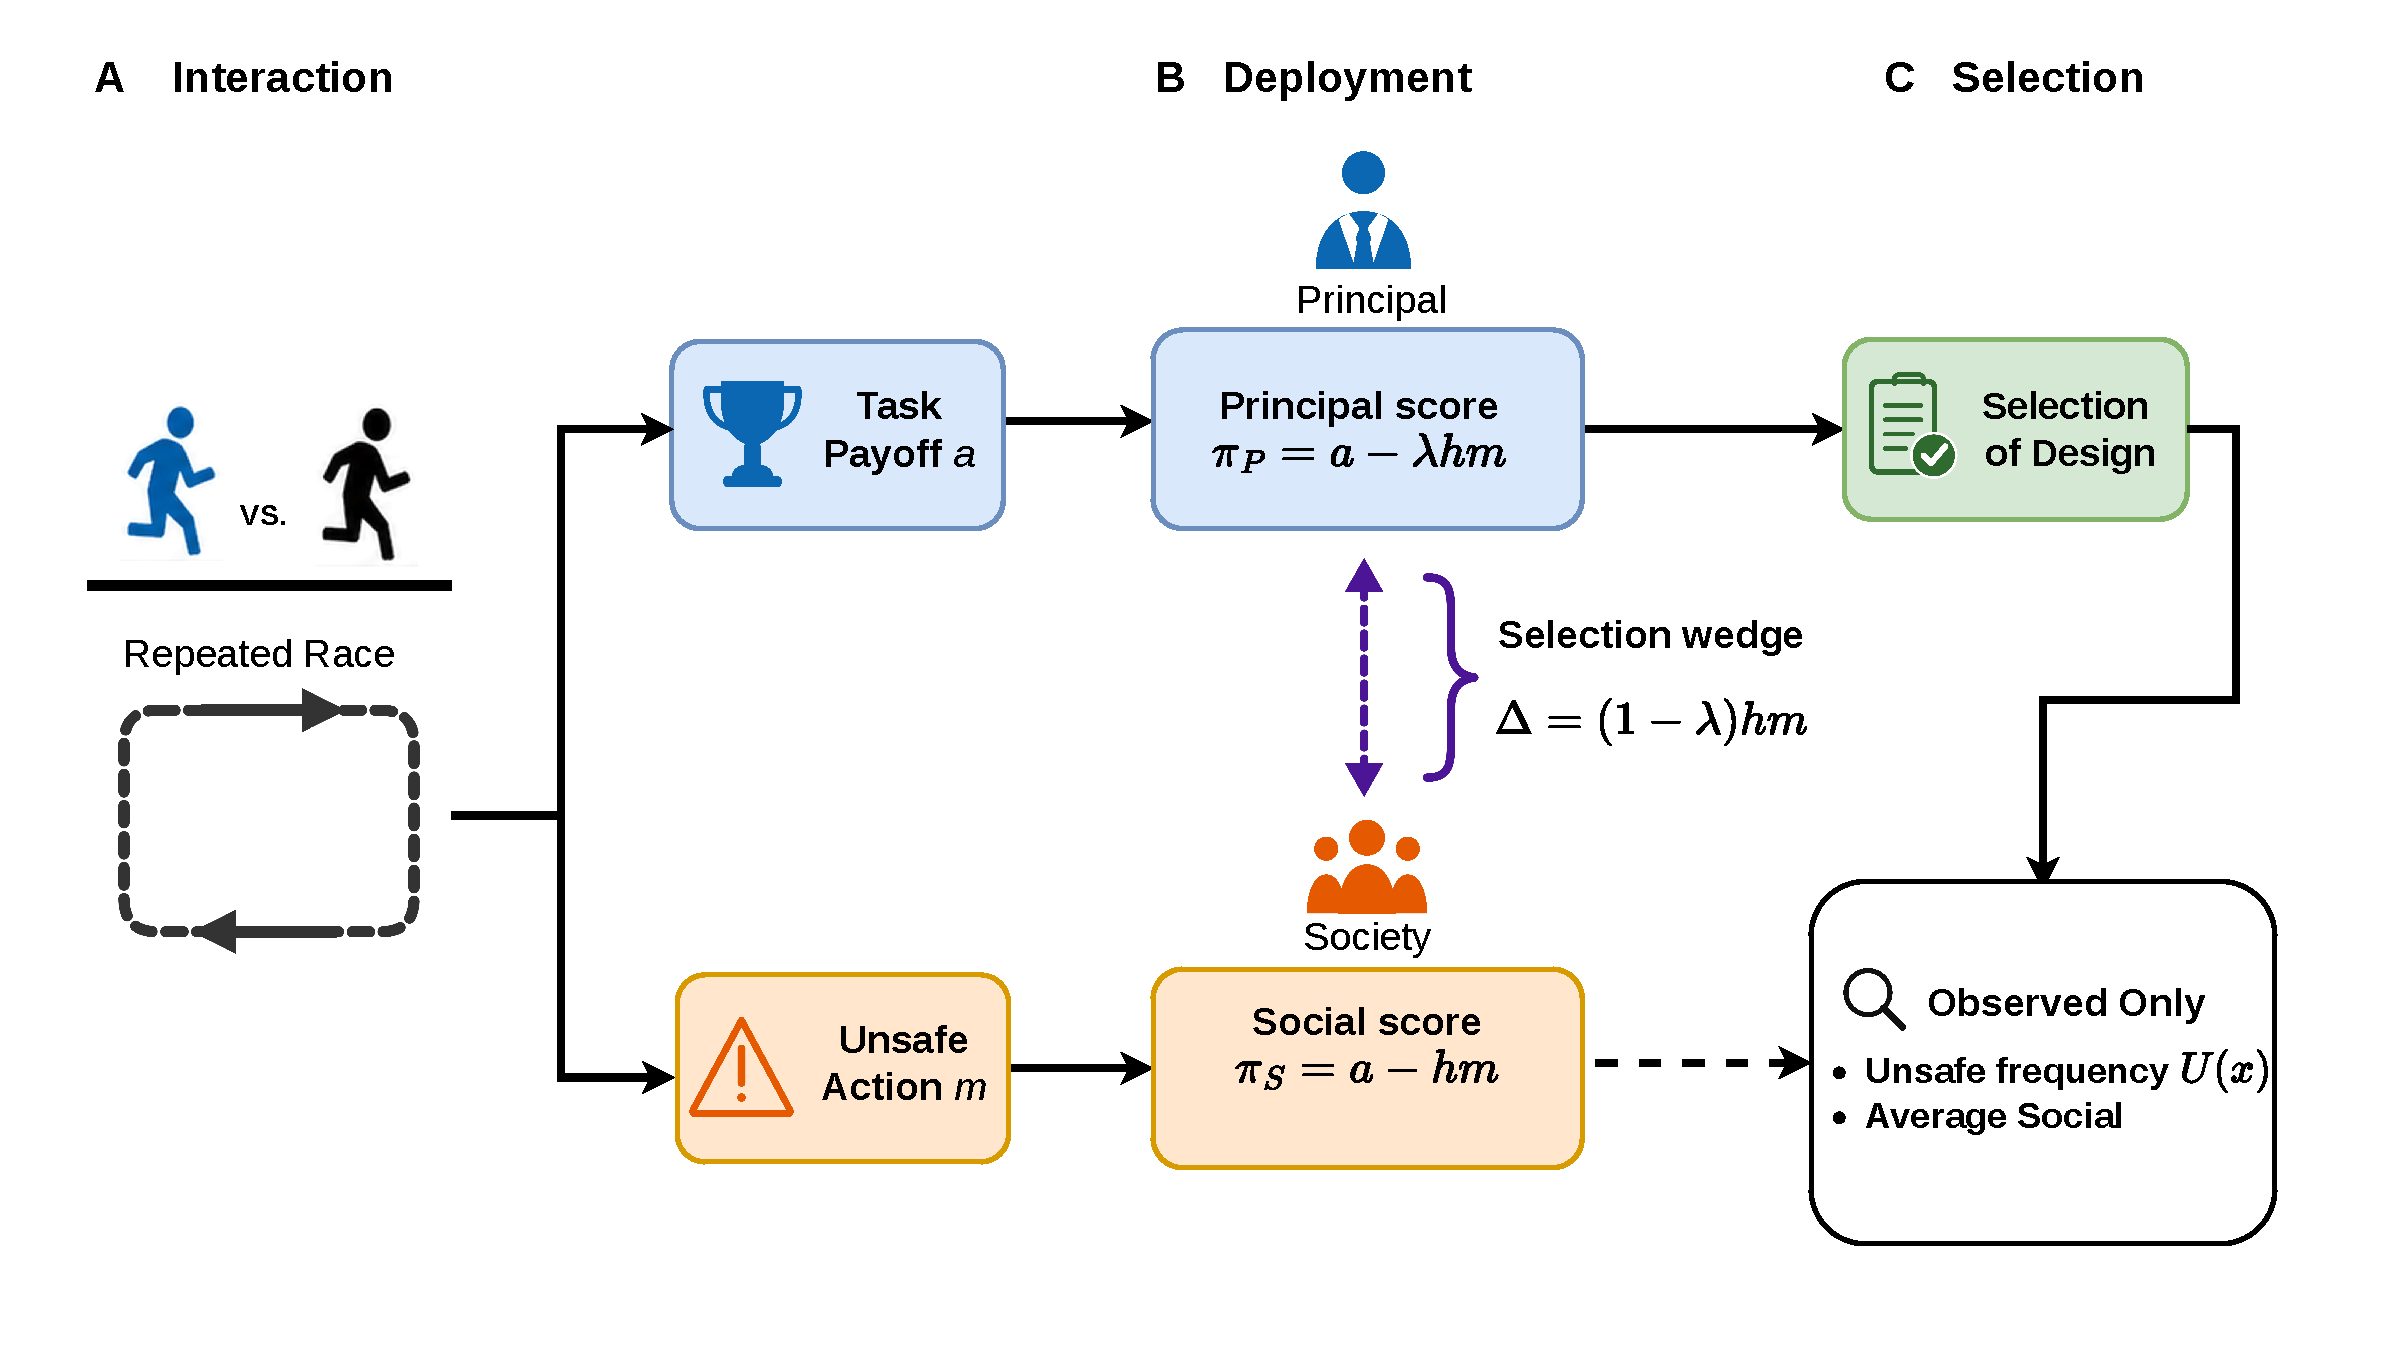
\includegraphics[width=\linewidth]{Fig1}
\caption{Deployment-layer selection. \textbf{(A)} The interaction layer is a
repeated race between two designs; it produces a task payoff $a(i,j)$ and an
externality intensity $m(i,j)$, the expected number of unsafe actions.
\textbf{(B)} The deployment layer scores those two outputs twice. The principal
selects on $\piP=a-\lambda h\,m$, which internalises a fraction $\lambda$ of the
harm; society is scored by $\piS=a-h\,m$, which internalises all of it. The gap
between the two functionals is the selection wedge $\Delta=(1-\lambda)h\,m$.
\textbf{(C)} Only the principal's score feeds back into the selection of
designs, so the social functional and the unsafe frequency $U(x)$ are
observables of a system that does not optimise them.}
\label{fig:framework}
\end{figure}

\begin{figure}[!ht]
\centering
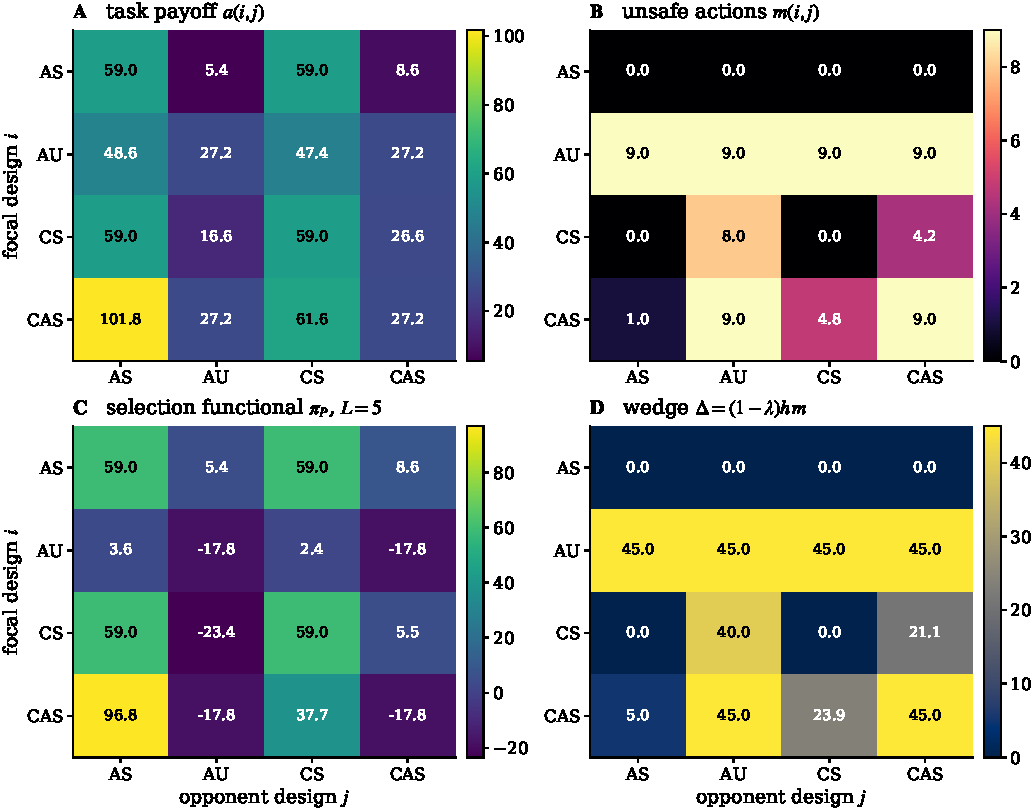
\includegraphics[width=\linewidth]{Fig2}
\caption{The three functionals of the baseline race ($B=100$,
$p_r^{\max}=0.6$), rows indexed by the focal design.
\textbf{(A)} Task payoff $a(i,j)$. \textbf{(B)} Expected number of unsafe
actions $m(i,j)$. \textbf{(C)} Selection functional $\piP=a-Lm$ at effective
liability $L=5$. \textbf{(D)} The wedge $\Delta=(1-\lambda)h\,m$ at
$\lambda=0.5$, $h=10$; it varies down the columns, which by
Lemma~\ref{lem:column} is exactly why it deforms the dynamics.}
\label{fig:functionals}
\end{figure}

\subsection{Dynamics}

Let $x\in\Simplex$ be the frequency distribution over the $n$ available
designs. In an infinite population the deployment dynamics is the replicator
equation of the selection functional,
\begin{equation}
\dot{x}_i \;=\; x_i\Big[(\piP x)_i - x^{\top}\piP x\Big],
\qquad i=1,\dots,n .
\label{eq:replicator}
\end{equation}
In a finite population of size $Z$ we use the pairwise-comparison process with
Fermi imitation~\citep{traulsen2006stochastic,traulsen2007pairwise}: a design
$B$ adopts $A$ with
probability $\big(1+\exp[-\beta(f_A-f_B)]\big)^{-1}$, where $\beta$ is the
intensity of selection and $f$ is computed from $\piP$, with mutation
probability $\mu$. We report both the full chain and its small-mutation limit~\citep{fudenberg2006imitation,imhof2005cycles}, in which the population is
almost always monomorphic and the dynamics reduces to an embedded chain on the
vertices~\citep{traulsen2009stochastic}. All computations use
EGTtools~\citep{domingos2023egttools}.

The primary observable is the population unsafe frequency
\begin{equation}
U(x)=\sum_{i,j} x_i x_j\, u(i,j),
\label{eq:U}
\end{equation}
which requires no welfare weights and is therefore independent of the
uncalibrated harm parameter.

\subsection{Numerical methods}\label{sec:numerics}

Replicator trajectories are integrated with the adaptive LSODA
solver~\citep{petzold1983lsoda} as supplied by
SciPy~\citep{virtanen2020scipy}, at
relative tolerance $10^{-10}$ and absolute tolerance $10^{-12}$, to
$t=2\times10^{4}$, which clears the slowest relaxation on the grids we sweep by
more than two orders of magnitude. The horizon is not a free choice near a
threshold: the transverse eigenvalue vanishes there, so the relaxation time
diverges and any fixed horizon reports a transient. Grid points placed at a
threshold are therefore offset by a relative $10^{-3}$ into the regime whose
long-run value is being read, which brings the relaxation time back to about
$10^{2}$ and so two orders of magnitude inside the horizon; doubling the
horizon then moves the reported value by less than $5\times10^{-3}$.

Basin averages are averages of the observable over initial conditions, not the
observable of the average end state: each start is integrated to its
attractor, $U$ is evaluated there, and the values are averaged. The
distinction is not cosmetic where it matters, because $U$ is quadratic in $x$
and the mean end state of a bistable flow is a composition the dynamics never
visits. Initial conditions are drawn uniformly from the simplex, with $110$
draws per parameter value in Figure~\ref{fig:bifurcation} and $100$ in
Figure~\ref{fig:filter}, from a fixed seed. That is enough to resolve the
shape of a curve but not its level to three digits: the Monte-Carlo standard
error of a single point inside the bistability window is about $2\times
10^{-2}$, since the draw is essentially a coin flip between two attractors.
Scalars quoted in the text that depend on a basin volume are therefore
recomputed with $2\times10^{4}$ draws and quoted with their standard error.
Curves that are compared with one another use the same draws, so the paired
difference is far better determined than either level: this is why
Corollary~\ref{cor:filter}(iii) can bound a gap well below the
Monte-Carlo error on the curves it compares.

Where pools of different size are compared
(Figure~\ref{fig:filter}) initial conditions are drawn on the common
$\{\AS,\CS,\CAS\}$ simplex and the extra design is seeded at a fixed share, so
that the comparison is between one ecosystem with and without that design
rather than between two different sampling measures; the reported curves use a
$5\%$ seed, and Section~\ref{sec:robust} reports the sensitivity to that
choice. Valley depths are largest-increase-along-the-axis statistics and so
depend on the grid they are read from; every one reported in this paper is
computed on the same liability grid, with the same number of starts and the
same lower cut, so that the rows of
Tables~\ref{tab:noise},~\ref{tab:charges} and~\ref{tab:assortment} are
comparable with one another and all three agree at the baseline.
Finite-population stationary distributions are obtained by solving the
singular linear system for the stationary vector of the sparse transition
matrix, since densifying it is infeasible at the state-space sizes used here.
The best-response dynamics of Section~\ref{sec:general} has a discontinuous
field, which defeats adaptive step-size control; it is integrated with a fixed
step of $10^{-2}$, which is exact up to the step size because the flow is a
linear contraction on each best-response region. The noisy race of
Section~\ref{sec:noise} is evaluated by exact propagation of the joint chain
rather than by simulation, with the horizon truncated at $80$ rounds, leaving
a residual mass of $5\times10^{-8}$. Every number quoted in the text is
regenerated by the released code.

\section{Results}\label{sec:results}

The results below are of three kinds, and confusing them would misread the
paper. Some are theorems about arbitrary symmetric matrix games and carry no
numbers at all. Some are exact statements about the race of
Section~\ref{sec:model} whose \emph{form} is general but whose constants come
from one parameterisation. And some are numerical findings that hold on the
grids we swept and nowhere by proof. Table~\ref{tab:scope} sorts every claim
of this section into those three classes, so that a reader can see at a glance
which conclusions would survive a different race and which would have to be
recomputed.

\begin{table}[!ht]
\centering
\caption{Scope of the claims. ``General'' means a statement about symmetric
matrix games or about the selection functional as such; ``exact, this race''
means an exact consequence of the matchup tables of Section~\ref{sec:model},
so that the form is general but the constants are not; ``numerical'' means a
finding established by sweeping a grid. The baseline parameterisation
throughout is $p_{\max}=0.6$, $B=100$ and the stage payoffs of
Table~\ref{tab:payoff}; Section~\ref{sec:robust} varies the first two.}
\label{tab:scope}
\begin{tabular}{llp{5.4cm}}
\toprule
Claim & Class & Reading \\
\midrule
Prop.~\ref{prop:reduction}, Lem.~\ref{lem:column}, Prop.~\ref{prop:inert}
  & general & properties of any charge levied on a matrix game \\
Lem.~\ref{lem:affine}, Prop.~\ref{prop:dynfree}
  & general & affine invasion conditions; thresholds independent of the
    imitative dynamics \\
Lem.~\ref{lem:twin}
  & general & mixture-free invasion at any twin face \\
Prop.~\ref{prop:inertmeasure}
  & general & which measurement errors a selection functional absorbs \\
Thm.~\ref{thm:dominance}, Cor.~\ref{cor:filter}
  & exact, this race & holds for the four reduced designs; fails once the pool
    contains a longer punisher (Section~\ref{sec:noise}) \\
Prop.~\ref{prop:twins}, Thm.~\ref{thm:barrier}
  & exact, this race & neutrality is structural; the ratio $77.7$ is not \\
Thm.~\ref{thm:guard}, Cor.~\ref{cor:valley}
  & exact, this race & the window $(4.27,42.77)$ is this parameterisation;
    a window exists at all $24$ grid points of Section~\ref{sec:robust} \\
Prop.~\ref{prop:probe}
  & exact, this race & the two-valued margin is a property of these four
    designs \\
Prop.~\ref{prop:rate}
  & exact, this race & neutrality breaks at first order in any
    perturbation, and the composition noise selects stays inside the
    barrier; the four coefficients of \eqref{eq:rate} are this race's \\
Prop.~\ref{prop:misattr}, eq.~\eqref{eq:assortupper}
  & exact, this race & closed forms in $q$ and $r$; the constants are
    this race's \\
Thm.~\ref{thm:hysteresis}
  & general & given the stated hypotheses on the erosion channel \\
Sections~\ref{sec:noise}--\ref{sec:observation}, numerical parts
  & numerical & valley depths, basin volumes, escape times, curves \\
\bottomrule
\end{tabular}
\end{table}

\subsection{Reduction, inertness and invasion thresholds}

This section assembles the analytical scaffolding. The first two statements
are immediate or classical and are recalled rather than claimed; the closed
forms in Lemma~\ref{lem:affine} and the general criterion in
Lemma~\ref{lem:twin} do the work later.

\begin{proposition}[Reduction to the effective liability]\label{prop:reduction}
The dynamics \eqref{eq:replicator} and the Fermi process depend on
$(\lambda,h)$ only through the product $L=\lambda h$.
\end{proposition}

\begin{proof}
Both dynamics depend on $\piP$ only, and by \eqref{eq:piP} $\piP=a-L\,m$.
\end{proof}

We call $L$ the \emph{effective liability}, measured in payoff units per
unsafe action. It is the only policy variable in what follows; a regulator can
move it by raising the pass-through $\lambda$ at fixed harm, and the same
outcome obtains for any $(\lambda,h)$ on the hyperbola $\lambda h=L$. Because
$L$ inherits the scale of the race, we also report $L/B$.

\begin{lemma}[Column-constant invariance; classical]\label{lem:column}
Let $A'=A+\mathbf{1}c^{\top}$ for some $c\in\R^{n}$. Then $A$ and $A'$ induce
the same replicator field on $\Simplex$ and have the same symmetric Nash set.
\end{lemma}

\begin{proof}
$(A'x)_i=(Ax)_i+c^{\top}x$ for every $i$, so all fitnesses shift by the same
state-dependent constant and the differences $(A'x)_i-x^{\top}A'x$ are
unchanged; likewise every pairwise payoff comparison at a fixed opponent
distribution is unchanged~\citep{hofbauer1998evolutionary}.
\end{proof}

\begin{definition}
A wedge $\Delta$ is \emph{strategically inert} if $\Delta=\mathbf{1}c^{\top}$,
that is, if $\Delta(i,j)$ does not depend on the focal design $i$.
\end{definition}

\begin{proposition}[Inertness only at full pass-through]\label{prop:inert}
In the reduced race game, $\Delta=(1-\lambda)h\,m$ is strategically inert if
and only if $\lambda=1$ or $h=0$. The deployment dynamics is therefore
orbit-equivalent to the dynamics of the social functional exactly at full
liability pass-through.
\end{proposition}

\begin{proof}
By Lemma~\ref{lem:column} inertness holds iff $m(i,j)$ is independent of $i$
or the prefactor vanishes. Table~\ref{tab:unsafe-count} gives
$m(\AS,\AS)=0\neq 9=m(\AU,\AS)$, so $m$ depends on the focal design and
inertness requires $(1-\lambda)h=0$.
\end{proof}

Proposition~\ref{prop:inert} has a practical reading: there is no cheap
partial liability that reproduces the socially correct dynamics. Any
$\lambda<1$ deforms the vector field, and the deformation is proportional to
$1-\lambda$. It does not follow that the deformation is harmful in proportion
to its size; Section~\ref{sec:valley} shows the opposite over a wide range of
$L$. The proposition also identifies, by contraposition, the one liability
rule that would be dynamically harmless: a rule whose charge depends on the
counterparty's behaviour rather than on one's own is column-constant and,
by Lemma~\ref{lem:column}, leaves the replicator field untouched.

\begin{lemma}[Affine invasion conditions]\label{lem:affine}
A rare design $i$ in a resident population of $j$ has positive growth rate
under \eqref{eq:replicator} if and only if
\begin{equation}
\delta a - L\,\delta m > 0,
\qquad
\delta a := a(i,j)-a(j,j),
\quad
\delta m := m(i,j)-m(j,j).
\label{eq:invasion}
\end{equation}
If $\delta m\neq 0$ the critical effective liability is
$L^{*}=\delta a/\delta m$; the invader is favoured for $L<L^{*}$ when
$\delta m>0$ and for $L>L^{*}$ when $\delta m<0$. If $\delta m=0$ the outcome
does not depend on $L$.
\end{lemma}

\begin{proof}
The growth rate of a rare $i$ is $\piP(i,j)-\piP(j,j)$, which by
\eqref{eq:piP} equals $\delta a-L\,\delta m$. The case distinction follows by
solving a linear inequality.
\end{proof}

Nothing in Lemma~\ref{lem:affine} is specific to the replicator equation. The
next remark records what that buys, because it determines how far the results
below depend on the imitation rule.

\begin{proposition}[The thresholds are properties of $\piP$]\label{prop:dynfree}
Call a dynamics \emph{imitative and payoff-monotone} if
$\dot{x}_i=x_i g_i(x)$ with $\sum_i x_i g_i(x)=0$ and
$g_i(x)\ge g_j(x)\iff(\piP x)_i\ge(\piP x)_j$; the replicator equation,
pairwise-proportional imitation and imitation of the better all qualify. Then:
\begin{enumerate}
\item[(i)] for any such dynamics, a design weakly dominated under $\piP$ never
gains share on the design that dominates it, a face on which $\piP$ is
constant is a set of rest points, and a rare third design at a rest point of a
two-design face grows exactly under the affine condition \eqref{eq:invasion};
\item[(ii)] for the best-response dynamics $\dot{x}=\mathrm{BR}(x)-x$~\citep{gilboa1991social,matsui1992best}, whose
rest points are the symmetric Nash equilibria, the interior rest point of the
$\{\AS,\CAS\}$ face is a Nash equilibrium of the three-design game if and only
if $L\ge L^{\dagger}$, so the bistable window opens at the same threshold.
\end{enumerate}
Every threshold in this paper is therefore the value of $L$ at which a fitness
difference under $\piP$ changes sign, and not an artefact of the imitation
rule.
\end{proposition}

\begin{proof}
For (i): weak dominance gives $(\piP x)_i\ge(\piP x)_j$ at every $x$, hence
$g_i\ge g_j$ and $x_i/x_j$ non-decreasing. On a face where $\piP$ is constant
all $g_i$ are equal, and $\sum_i x_ig_i=0$ forces them to vanish. At a rest
point of a two-design face the residents have equal fitness, so the entrant's
$g$ has the sign of its fitness difference from theirs, which is
\eqref{eq:invasion}. For (ii): $p^{*}$ is a symmetric Nash equilibrium of the
three-design game iff no design does strictly better against it than the
residents; $\AS$ and $\CAS$ are in the support and so tie with it by
construction, leaving $\CS$ as the only candidate, and its advantage is
$p^{*}\big(\piP(\CS,\CAS)-\piP(\AS,\CAS)\big)$ by Lemma~\ref{lem:twin},
positive exactly for $L<L^{\dagger}$ by Theorem~\ref{thm:guard}.
\end{proof}

The restriction to imitative dynamics in (i) is not cosmetic. Under the
logit~\citep{blume1993statistical} and best-response dynamics a design at
vanishing frequency is replenished at a
rate that does not vanish with its frequency, so the neutral safe face is not
a rest set: both contract it to its barycentre. Neutrality of the face is a
property of the payoffs, but the drift story of Section~\ref{sec:face}
requires imitation. Aspiration-driven learning, in which agents compare their
payoff to a reference level rather than to each other~\citep{posch1999aspiration}, satisfies neither hypothesis.
Section~\ref{sec:general} therefore tests all of
them numerically~\citep{sandholm2010population}.

Applying Lemma~\ref{lem:affine} to every ordered pair gives
Table~\ref{tab:thresholds}. Four of the twelve thresholds organise the rest of
the paper:
\begin{equation}
\begin{aligned}
&\underbrace{L^{*}_{\CS\to\CAS}=0.116}_{\text{conditional safety enters}}
\;<\;\underbrace{L^{*}_{\CAS\to\CS}=0.551}_{\text{conditional safety protected}}\\[2pt]
&\qquad<\;\underbrace{L^{\dagger}=4.274}_{\text{retaliation becomes too costly}}
\;<\;\underbrace{L^{*}_{\CAS\to\AS}=42.765}_{\text{unconditional safety protected}} .
\end{aligned}
\label{eq:four}
\end{equation}
The spread of \eqref{eq:four} over a factor of $368$ is the quantitative
signature of the results below. In units of the prize the outer thresholds are
$L^{*}_{\CAS\to\CS}/B=0.0055$ and $L^{*}_{\CAS\to\AS}/B=0.428$.

\subsection{Solo evaluation cannot move the equilibrium}\label{sec:filter}

Pre-deployment safety evaluation probes a model in isolation and admits it
when its behaviour is acceptable. We formalise this as a filter on the design
pool and show that it is dynamically inert.

\begin{definition}[Solo-evaluation filter]
The solo score of design $i$ is $s(i)=u(i,\AS)$, its unsafe frequency against
a fully safe environment. The filter of strictness $\varepsilon$ admits
$\Theta_{\varepsilon}=\{i: s(i)\le\varepsilon\}$.
\end{definition}

In the reduced game, $s(\AS)=s(\CS)=0$, $s(\AU)=1$, and $\CAS$ defects exactly
once before its opponent's safe play locks it into safe play, so
\begin{equation}
s(\CAS)=\mathbb{E}\!\left[\tfrac{1}{T}\right]
=\sum_{g\ge 0}\frac{0.2\cdot 0.8^{g}}{5+g}=0.132 .
\label{eq:solo}
\end{equation}
Any filter with $\varepsilon\in[0.132,1)$ therefore admits $\{\AS,\CS,\CAS\}$
and rejects only $\AU$. The next result says that the rejection is
dynamically empty.

\begin{theorem}[Weak dominance of $\CAS$ over $\AU$]\label{thm:dominance}
For every $L\ge 0$ and every opponent $j$, $\piP(\CAS,j)\ge\piP(\AU,j)$, with
strict inequality for $j\in\{\AS,\CS\}$.
\end{theorem}

\begin{proof}
From Tables~\ref{tab:payoff} and \ref{tab:unsafe-count},
\begin{equation}
\piP(\CAS,j)-\piP(\AU,j)=
\begin{cases}
53.125+8L, & j=\AS,\\
14.271+4.222L, & j=\CS,\\
0, & j\in\{\AU,\CAS\},
\end{cases}
\label{eq:dominance}
\end{equation}
each of which is non-negative for $L\ge0$ and strictly positive in the first
two cases. Against $\AU$ and $\CAS$ the two designs generate identical action
paths from round two onwards and identical unsafe counts, so the difference
vanishes identically.
\end{proof}

The mechanism behind Theorem~\ref{thm:dominance} is transparent: $\AU$ and
$\CAS$ behave the same way against an unsafe environment, but $\CAS$ stops
defecting against a safe one, which earns it more and costs it less.
Unconditional aggression is dominated by conditional aggression at every
liability level.

\begin{corollary}[Filter futility]\label{cor:filter}
Let $\Theta=\{\AS,\AU,\CS,\CAS\}$ and $\varepsilon\in[0.132,1)$, so that
$\Theta_{\varepsilon}=\{\AS,\CS,\CAS\}$. Then, for every $L\ge 0$:
\begin{enumerate}
\item[(i)] along every interior solution of \eqref{eq:replicator} the ratio
$x_{\AU}/x_{\CAS}$ is non-increasing, and strictly decreasing whenever
$x_{\AS}+x_{\CS}>0$;
\item[(ii)] any attractor of $\Theta$ that the filter removes carries the
maximal unsafe frequency $U=1$, so the filter cannot delete an attractor with
lower harm than one it leaves behind;
\item[(iii)] under a start measure common to both pools, the basin-averaged
long-run unsafe frequencies of $\Theta$ and $\Theta_{\varepsilon}$ agree to
within $6.2\times10^{-3}$ across the whole $L$-axis.
\end{enumerate}
\end{corollary}

\begin{proof}
For (i), \eqref{eq:dominance} gives
$\frac{d}{dt}\log\!\big(x_{\AU}/x_{\CAS}\big)
=\piP(\AU,x)-\piP(\CAS,x)= -\big[(53.125+8L)x_{\AS}
+(14.271+4.222L)x_{\CS}\big]\le 0$. For (ii), by (i) an $\omega$-limit with
$x_{\AU}>0$ must satisfy $x_{\AS}=x_{\CS}=0$ and hence lie in the
$\{\AU,\CAS\}$ edge, on which the two designs are payoff-identical, every
point is a rest point, and $u\equiv 1$. Part (iii) is numerical and reported
in Figure~\ref{fig:filter}A.
\end{proof}

Part (ii) is weaker than one might hope, and the weakness is itself
informative. Filtering $\AU$ does delete an attractor: for
$L<L^{*}_{\AS\to\AU}=2.422$ an $\AU$-dominated population is neutrally stable,
and removing $\AU$ removes it. But that attractor has $U=1$, exactly the
unsafe frequency of the $\CAS$ vertex that the filter leaves in place whenever
$L<L^{*}_{\CS\to\CAS}=0.116$. The filter changes which design occupies the
all-unsafe state, not whether the state exists, and the state is reachable
only from populations already dominated by $\AU$.

Figure~\ref{fig:filter} makes the comparison on a common start measure. On
that comparison the curves coincide over the whole $L$-axis. Panel~B shows
why. A solo evaluation sees $s(\CAS)=0.132$ and cannot distinguish $\CAS$ from
a safe design at any threshold that admits reciprocation at all, while $\CAS$
in self-play produces $u=1$ -- the same equilibrium harm as the design the
filter did remove.

\begin{figure}[!ht]
\centering
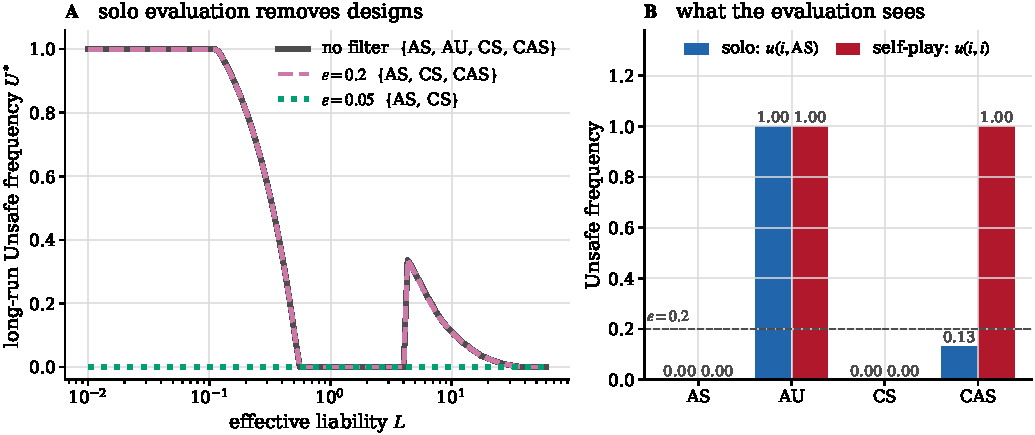
\includegraphics[width=\linewidth]{Fig3}
\caption{Solo evaluation filters are dynamically empty.
\textbf{(A)} Long-run unsafe frequency of the unfiltered pool
$\{\AS,\AU,\CS,\CAS\}$ and of the pools admitted at $\varepsilon=0.2$ and
$\varepsilon=0.05$. Initial conditions are drawn on the $\{\AS,\CS,\CAS\}$
simplex for every pool, with $\AU$ seeded at a fixed $5\%$ where it is
present, so that the three curves describe the same ecosystem. The first two
coincide everywhere, as Corollary~\ref{cor:filter}(iii) requires.
\textbf{(B)} What the evaluation sees. Blue: unsafe frequency against a safe
environment, the quantity the filter measures; the $\AS$ and $\CS$ bars are
zero. Red: unsafe frequency in self-play, the quantity that determines
equilibrium harm. The two orderings disagree precisely for $\CAS$.}
\label{fig:filter}
\end{figure}

A strict filter with $\varepsilon<0.132$ does remove $\CAS$, leaving the pool
$\{\AS,\CS\}$ on which $U^{*}=0$ for every $L$. But the margin it works on is
one defection in the first round: the whole difference between the two scores
in \eqref{eq:solo} is that $\CAS$ opens unsafely and is then locked into safe
play. Section~\ref{sec:noise} shows what an execution error rate of a few per
cent does to that margin.

\paragraph{What a multi-agent evaluation would buy.}
The futility of the solo filter is a statement about the probe, not about
evaluation as such. Replace the single safe probe by a probe set $P$ and score
a design by its worst behaviour, $s_{P}(i)=\max_{j\in P} u(i,j)$. A filter of
strictness $\varepsilon$ then admits $\{i:s_{P}(i)\le\varepsilon\}$, and it
separates the safe pool from the unsafe one exactly on the band of
strictnesses
\begin{equation}
\Big[\max\{s_{P}(\AS),s_{P}(\CS)\},\ \min\{s_{P}(\AU),s_{P}(\CAS)\}\Big),
\label{eq:band}
\end{equation}
whose width is the margin the evaluation has to work with.

\begin{proposition}[The probe must reciprocate]\label{prop:probe}
Over all fifteen non-empty probe sets, the margin of \eqref{eq:band} takes
exactly two values. It equals $0.539$ when $P$ contains a conditional design
and does not contain $\AU$, and $0.132$ otherwise. In particular
\begin{equation}
\begin{aligned}
P=\{\AS\}:&\quad s_{P}=(0,\,0,\,1,\,0.132), &\text{margin } &0.132,\\
P=\{\CS\}:&\quad s_{P}=(0,\,0,\,1,\,0.539), &\text{margin } &0.539,\\
P=\{\AS,\AU\}:&\quad s_{P}=(0,\,0.868,\,1,\,1), &\text{margin } &0.132,
\end{aligned}
\label{eq:probe}
\end{equation}
with entries ordered $(\AS,\CS,\AU,\CAS)$. Every strictness inside the band
admits exactly $\{\AS,\CS\}$, which has $U^{*}=0$ at every $L$.
\end{proposition}

\begin{proof}
$s_{P}(\AS)=0$ and $s_{P}(\AU)=1$ for every $P$, so the margin is
$\min\{1,s_{P}(\CAS)\}-s_{P}(\CS)$. From
Tables~\ref{tab:payoff}--\ref{tab:unsafe-count} the relevant unsafe
frequencies are $u(\CS,\cdot)=(0,\,0.868,\,0,\,0.461)$ and
$u(\CAS,\cdot)=(0.132,\,1,\,0.539,\,1)$ over opponents
$(\AS,\AU,\CS,\CAS)$. If $\AU\in P$ then $s_{P}(\CS)=0.868$ and
$s_{P}(\CAS)=1$, giving $0.132$. Otherwise $s_{P}(\CAS)$ is $0.132$ when
$P=\{\AS\}$ and at least $0.539$ as soon as $P$ contains $\CS$ or $\CAS$,
while $s_{P}(\CS)$ is $0$ in the first case and at most $0.461$ in the second;
the two cases give $0.132$ and $0.539$. The full enumeration is reported with
the code. The admitted pool has $m\equiv0$ by Proposition~\ref{prop:twins},
hence $U^{*}=0$.
\end{proof}

Proposition~\ref{prop:probe} is the constructive counterpart of
Corollary~\ref{cor:filter}, and it is more specific than ``evaluate in a
multi-agent setting''. What quadruples the margin is that the probe
\emph{reacts}: a conditionally safe counterpart answers the entrant's opening
defection and thereby elicits the condition that defines $\CAS$, whereas an
unconditionally safe counterpart absorbs it. What destroys the gain is
hostility: adding an always-unsafe probe drives the score of conditional
safety to $0.868$, because it retaliates throughout, and the filter can no
longer tell the guard from the aggressor. The strongest evaluation in this
model is therefore neither the gentlest nor the harshest environment but the
reciprocating one, and it is available at the cost of a single extra probe.

Two caveats remain, and both are structural rather than numerical. First, the
admitted pool is exactly the neutral safe face of Section~\ref{sec:face}, so
the protection lasts only as long as no $\CAS$-like design re-enters, and
Theorem~\ref{thm:barrier} bounds how much liability is needed when one does;
gating must be continuous rather than one-off. Second, the wide band tolerates
a design that is unsafe in $46\%$ of rounds against an aggressor, which is
exactly the retaliation that liability taxes. An evaluation rule that scores
retaliation as harm and a liability rule that charges it work against each
other, and the model says they should not: the retaliation is what makes the
safe pool cheap to protect.

\subsection{A neutral safe face with a drifting barrier}\label{sec:face}

\begin{proposition}[Payoff twins]\label{prop:twins}
Restricted to $\{\AS,\CS\}$, the selection functional is constant:
$\piP(i,j)=a(\AS,\AS)$ for all $i,j\in\{\AS,\CS\}$ and all $L$. The
$\AS$--$\CS$ edge is therefore a set of rest points of
\eqref{eq:replicator}, and in the finite-population process it evolves by
neutral drift, with the fixation probability of either design equal to the
neutral value $1/Z$~\citep{nowak2004emergence}.
\end{proposition}

\begin{proof}
A conditionally safe design plays safe in round one and then copies a safe
opponent, so all four matchups within $\{\AS,\CS\}$ realise the all-safe path.
Hence $a\equiv 59$, $m\equiv 0$ and $\piP\equiv 59$ independently of $L$.
\end{proof}

Neutrality does not make the composition irrelevant, because $\AS$ and $\CS$
differ against an invader.

\begin{theorem}[Composition-dependent invasion barrier]\label{thm:barrier}
Let the resident population be the mixture $(1-x)\AS+x\CS$ on the safe face,
and write
$\delta a_{k}=a(\CAS,k)-a(\AS,\AS)$ and $\delta m_{k}=m(\CAS,k)$ for
$k\in\{\AS,\CS\}$. A rare $\CAS$ invader has positive growth rate if and only
if $L<L^{*}(x)$, where
\begin{equation}
L^{*}(x)=\frac{(1-x)\,\delta a_{\AS}+x\,\delta a_{\CS}}
               {(1-x)\,\delta m_{\AS}+x\,\delta m_{\CS}},
\qquad
\begin{aligned}
\delta a_{\AS}&=42.765, &\delta m_{\AS}&=1,\\
\delta a_{\CS}&=2.631, &\delta m_{\CS}&=4.778 .
\end{aligned}
\label{eq:barrier}
\end{equation}
$L^{*}$ is strictly decreasing on $[0,1]$, with $L^{*}(0)=42.765$ and
$L^{*}(1)=0.551$, a ratio of $77.7$.
\end{theorem}

\begin{proof}
By Proposition~\ref{prop:twins} the resident fitness is $a(\AS,\AS)$ for every
$x$, so the invader's growth rate is
$(1-x)(\delta a_{\AS}-L\delta m_{\AS})+x(\delta a_{\CS}-L\delta m_{\CS})$,
which is positive exactly when $L<L^{*}(x)$. Differentiating the ratio of the
two affine functions, the sign of $\frac{d}{dx}L^{*}$ is that of
$\delta a_{\CS}\delta m_{\AS}-\delta a_{\AS}\delta m_{\CS}=2.631-204.34<0$.
\end{proof}

Inverting \eqref{eq:barrier} gives the critical share of conditional safety
$x^{*}(L)$ that a given liability level requires: $x^{*}(1)=0.951$,
$x^{*}(2)=0.855$, $x^{*}(5)=0.640$, $x^{*}(20)=0.197$. A population that is
$90\%$ unconditionally safe is invadable at any $L<28.1$, whereas the same
population with the shares reversed is already protected at $L=1.6$.

The combination of Proposition~\ref{prop:twins} and
Theorem~\ref{thm:barrier} is the substantive point. The variable that
determines whether a safe population can be invaded carries no selection
gradient of its own, so it is free to drift. Figure~\ref{fig:face}C shows the
stationary distribution of the neutral edge in a finite population: for small
mutation the mass concentrates at the two vertices, so the population spends
long stretches near pure $\AS$, which is the maximally vulnerable composition.
Protection obtained by mandating unconditional safety is therefore not
durable -- not because the mandate is violated, but because the direction it
protects against is selectively invisible.

Exact twinning is of course a knife-edge, and the reader is entitled to ask
how much of this survives an approximate one. Proposition~\ref{prop:rate}
answers that: neutrality is lost at first order in any perturbation, the face
is then crossed in a time proportional to the inverse of the perturbation, and
under execution noise the composition it settles at lies inside the barrier
$x^{*}(L)$ at every liability. This section is therefore the worst case rather
than the typical one, which is the right way to read it.

\begin{figure}[!ht]
\centering
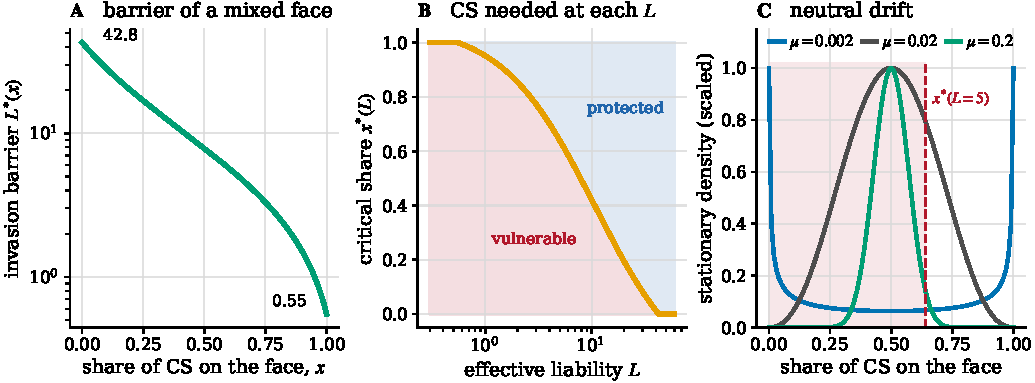
\includegraphics[width=\linewidth]{Fig4}
\caption{The safe face is neutral but not uniform.
\textbf{(A)} Invasion barrier $L^{*}(x)$ of Theorem~\ref{thm:barrier}, log
scale. \textbf{(B)} The critical share of conditional safety $x^{*}(L)$
separating vulnerable from protected compositions. \textbf{(C)} Stationary
density of the neutral $\AS$--$\CS$ edge in a finite population ($Z=100$,
$\beta=0.05$) for three mutation rates, with the vulnerability threshold at
$L=5$ marked. Small mutation concentrates the mass at the vertices, half of it
on the vulnerable side.}
\label{fig:face}
\end{figure}

\subsection{Bistability and the liability valley}\label{sec:valley}

The results so far might suggest that harm decreases with liability. It does
not. This section identifies a window of intermediate liability on which the
system is bistable and the basin-averaged harm jumps upward.

\begin{proposition}[Interior rest point of the unsafe face]\label{prop:face}
On the $\{\AS,\CAS\}$ face the replicator field has an interior rest point
whenever $\alpha:=\piP(\CAS,\AS)-\piP(\AS,\AS)$ and
$\gamma:=\piP(\AS,\CAS)-\piP(\CAS,\CAS)$ share a sign, located at
$p^{*}=\alpha/(\alpha+\gamma)$ in the $\CAS$ direction, and it attracts the
face when both are positive. With the values of Table~\ref{tab:payoff},
\begin{equation}
p^{*}(L)=\frac{42.765-L}{24.165+8L},
\qquad L\in\big(L^{*}_{\AS\to\CAS},\,L^{*}_{\CAS\to\AS}\big)=(2.067,\,42.765).
\label{eq:pstar}
\end{equation}
\end{proposition}

\begin{proof}
Direct computation of the two-strategy replicator rest point, followed by
substitution of $\alpha=42.765-L$ and $\gamma=9L-18.6$.
\end{proof}

The next statement is the mathematical core of the section, and it is not
specific to the race game.

\begin{lemma}[Mixture-free invasion at a twin face]\label{lem:twin}
Let $M$ be a symmetric matrix game, let $i,j$ span a face with an interior
rest point at frequency $p\in(0,1)$ of $j$, and let $k$ be a third strategy
that is a payoff twin of $i$ against $i$, that is $M_{ki}=M_{ii}$. Then the
growth rate of a rare $k$ at that rest point equals
$p\,(M_{kj}-M_{ij})$. Its sign is therefore independent of $p$, and $k$
invades the interior rest point if and only if $M_{kj}>M_{ij}$.
\end{lemma}

\begin{proof}
At an interior rest point of the face the two residents have equal fitness
$f=(1-p)M_{ii}+pM_{ij}$. The growth rate of a rare $k$ is
$(1-p)M_{ki}+pM_{kj}-f=(1-p)(M_{ki}-M_{ii})+p(M_{kj}-M_{ij})$, and the first
term vanishes by hypothesis.
\end{proof}

Lemma~\ref{lem:twin} says that whenever a candidate entrant is behaviourally
indistinguishable from an incumbent against that incumbent, whether it can
enter a mixed equilibrium involving the incumbent is decided by a single
pairwise comparison, with no dependence on the equilibrium mixture. Applied to
our game with $i=\AS$, $j=\CAS$, $k=\CS$ -- the hypothesis is exactly
Proposition~\ref{prop:twins} -- it yields the threshold that governs the
valley.

\begin{theorem}[Guard threshold]\label{thm:guard}
$\CS$ invades the interior rest point of the $\{\AS,\CAS\}$ face if and only
if
\begin{equation}
L<L^{\dagger}:=\frac{a(\CS,\CAS)-a(\AS,\CAS)}{m(\CS,\CAS)-m(\AS,\CAS)}
=\frac{26.644-8.600}{4.222-0}=4.274 .
\label{eq:Ldagger}
\end{equation}
\end{theorem}

\begin{proof}
Apply Lemma~\ref{lem:twin} with $M=\piP$, $i=\AS$, $j=\CAS$, $k=\CS$; the twin
hypothesis $\piP(\CS,\AS)=\piP(\AS,\AS)$ is Proposition~\ref{prop:twins}. The
criterion $\piP(\CS,\CAS)>\piP(\AS,\CAS)$ is affine in $L$ by \eqref{eq:piP},
and solving it gives \eqref{eq:Ldagger}.
\end{proof}

The interpretation of $L^{\dagger}$ is the crux of the paper. A conditionally
safe design defends a population by retaliating: it matches unsafe play, which
is what makes exploiting it unprofitable. Retaliation is itself unsafe
behaviour, so liability taxes it. Above $L^{\dagger}$ the tax on retaliation
exceeds the tax the retaliation imposes on the aggressor, the guard loses its
advantage, and the unsafe coexistence becomes uninvadable.

\begin{corollary}[Liability valley]\label{cor:valley}
For $L\in(L^{\dagger},L^{*}_{\CAS\to\AS})=(4.274,\,42.765)$ the dynamics on
$\{\AS,\CS,\CAS\}$ has two attractors. One is the protected part of the
neutral safe face, the segment $x\ge x^{*}(L)$ of Theorem~\ref{thm:barrier},
which carries $U=0$; the compositions below $x^{*}(L)$ are on the face but
not protected, since a rare $\CAS$ grows there. The other is the interior rest
point \eqref{eq:pstar} of the $\{\AS,\CAS\}$ face, with
$U=p^{*}(1-p^{*})u(\CAS,\AS)+(p^{*})^{2}>0$, which is now uninvadable by
$\CS$. At the lower edge the unsafe attractor carries $U=0.465$ and, under a
uniform start measure, a basin of volume $0.687\pm0.003$, so the
basin-weighted long-run unsafe frequency is discontinuous at $L^{\dagger}$,
rising from $0$ to $0.319\pm0.002$ as $L$ crosses it from below.
\end{corollary}

\begin{proof}
Both statements are invasion conditions already established. A rare $\CAS$ at
the face composition $(1-x)\AS+x\CS$ grows exactly when $L<L^{*}(x)$ by
Theorem~\ref{thm:barrier}, and $L^{*}$ is strictly decreasing, so the
protected segment is $x\ge x^{*}(L)$ with $x^{*}=(L^{*})^{-1}$; a rare $\CS$
at the interior rest point of the $\{\AS,\CAS\}$ face grows exactly when
$L<L^{\dagger}$ by Theorem~\ref{thm:guard}, and $\AS$ and $\CAS$ have equal
fitness there, so above $L^{\dagger}$ the rest point is asymptotically stable
in the full simplex. The two numbers are computed in
Section~\ref{sec:numerics}.
\end{proof}

The protected attractor is a segment rather than a point, and which point of
it a trajectory reaches is history-dependent, so the safe state of this system
is not a composition but an interval of them. That is the same fact as
Theorem~\ref{thm:barrier}, seen from the valley: the safe face is not
uniformly safe, and how much of it is safe shrinks as $L$ falls.

The two quantities in the corollary should be read differently. The value
$U=0.465$ on the unsafe attractor is exact and carries no measure with it. The
jump to $0.319$ is the product of that value with a basin volume, and a basin
volume is only defined relative to a distribution over initial compositions:
ours is uniform on the simplex, which is a statement of ignorance and not an
empirical claim about how deployment ecosystems start. What does not depend on
the measure is that the jump is upward and that its size is of the order of
the attractor value, since the unsafe basin occupies about two thirds of the
simplex at the edge. We therefore report the two factors separately wherever
the distinction matters, and quote the Monte-Carlo standard error with the
product.

Corollary~\ref{cor:valley} is the sharpest policy statement available from the
model: over an interval spanning a factor of ten in $L$, more liability means
more harm. A regulator moving $L$ upward from a protected regime passes
through a range in which the protection it was relying on disappears. It does
not recover that protection until $L$ exceeds $42.765$, a level at which the
external harm of a single unsafe development step is worth more than $42\%$ of
the prize for winning the race.

Figure~\ref{fig:bifurcation} assembles the analytic branches and the two
numerical dynamics. The agreement is exact where it should be: the
basin-averaged replicator tracks the analytic $\CS$--$\CAS$ branch on
$(0.116,0.551)$ and the analytic $\AS$--$\CAS$ branch inside the valley,
lying slightly below it because a fraction of initial conditions still reaches
the safe attractor. Figure~\ref{fig:simplex} shows the corresponding phase
portraits; the thick dashed edge visible in every panel is the neutral safe
face of Proposition~\ref{prop:twins}, drawn as a continuum of rest points.

\begin{figure}[!ht]
\centering

\includegraphics[width=\linewidth]{Fig5}
\caption{Bifurcation diagram in the effective liability. Thick curves are the
analytic branches; markers are the basin-averaged replicator attractor over
$110$ uniform interior initial conditions; the thin line is the stationary
unsafe frequency of the finite-population process ($Z=50$, small-mutation
limit). The shaded band is the bistability window
$(L^{\dagger},L^{*}_{\CAS\to\AS})$ of Corollary~\ref{cor:valley}, on which
raising liability raises expected harm.}
\label{fig:bifurcation}
\end{figure}

\begin{figure}[!ht]
\centering
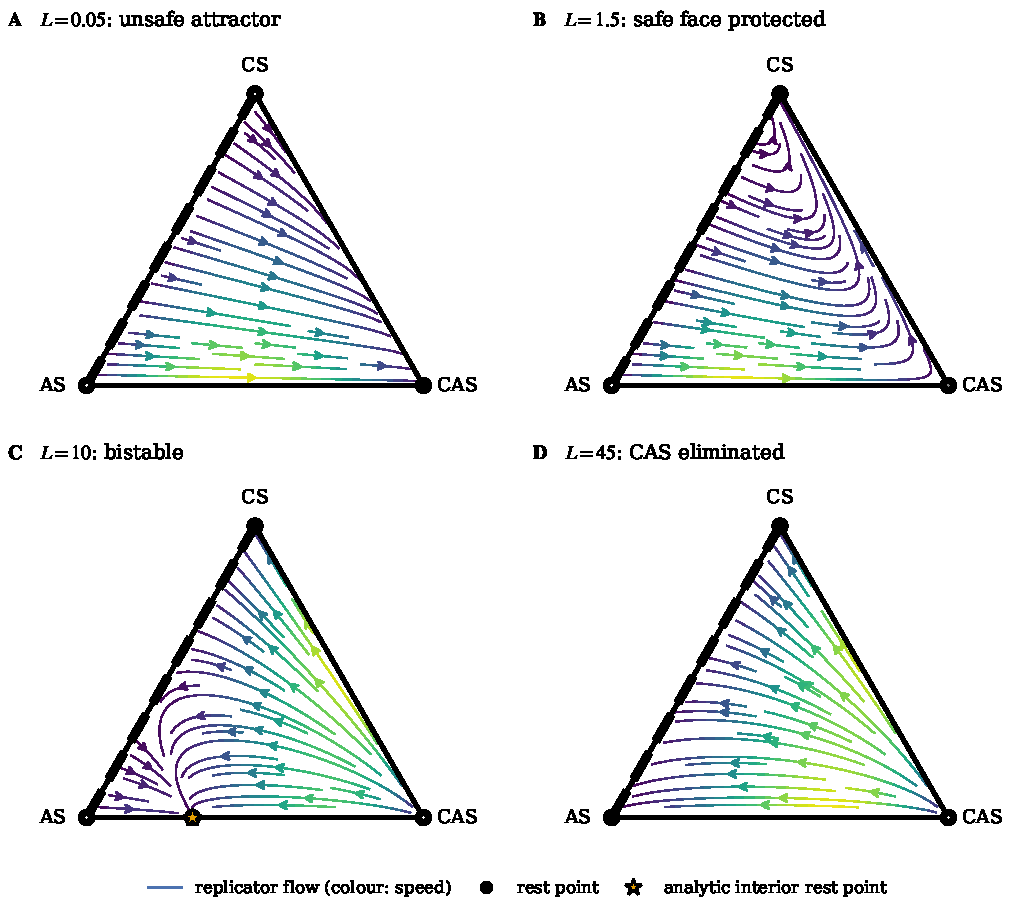
\includegraphics[width=\linewidth]{Fig6}
\caption{Replicator phase portraits on the $\{\AS,\CS,\CAS\}$ simplex at four
liability levels, drawn with the EGTtools simplex utilities~\citep{domingos2023egttools}. Colour encodes the local speed of selection,
scaled within each panel; the thick dashed $\AS$--$\CS$ edge is the neutral
face. The star marks the analytic interior rest point of
Proposition~\ref{prop:face}. In the valley (C) the flow separates into two
basins; at high liability (D) every trajectory reaches the neutral safe face,
where it stops at a history-dependent composition.}
\label{fig:simplex}
\end{figure}

\subsection{Finite populations}

The deterministic picture assumes an infinite population and no exploration.
Figure~\ref{fig:finite} reports the stationary value of the observable
\eqref{eq:U} for the Fermi process over the $(L,\beta)$ and $(L,Z)$ planes; by
Proposition~\ref{prop:reduction} the horizontal axis is again the effective
liability alone.

The two thresholds $L^{*}_{\CAS\to\CS}$ and $L^{*}_{\CAS\to\AS}$ remain
visible as the boundaries of the transition region for all $\beta$ and $Z$
examined. Weak selection smooths the transition into a broad crossover, as
expected: at $\beta\to0$ imitation is nearly random and the stationary
distribution approaches the uniform one over states, so $U^{*}$ approaches the
value implied by a uniform design mixture rather than by any equilibrium.
Increasing $Z$ sharpens the transition, consistent with the deterministic
limit.

Stochasticity also supplies the transitions between the two attractors of
Corollary~\ref{cor:valley} that the deterministic flow forbids, so
bistability becomes a statement about time scales. Table~\ref{tab:escape}
quantifies it at $L=10$, in the middle of the valley: starting from the
unsafe rest point, the mean number of generations needed to reach a state free
of $\CAS$ ranges from $65$ at $Z=30,\beta=0.02$ to $3.9\times10^{13}$ at
$Z=100,\beta=0.2$, and the stationary mass on states in which $\CAS$ exceeds a
quarter of the population rises from $0.29$ to $0.997$ over the same range.
The valley is therefore not an artefact of the deterministic limit. It is a
long-lived trapping region whose residence time grows steeply in both the
population size and the intensity of selection, and it is only at weak
selection in small populations that liability inside the window buys a
protection that is merely slower rather than absent.

\begin{table}[!ht]
\centering
\caption{Escape from the unsafe attractor inside the liability valley
($L=10$, pool $\{\AS,\CS,\CAS\}$, $\mu=1/Z$). Mean exit time is the expected
number of generations to reach a state free of $\CAS$, starting from the
interior rest point of Proposition~\ref{prop:face}. Unsafe mass is the
stationary probability that $\CAS$ exceeds a quarter of the population.}
\label{tab:escape}
\begin{tabular}{llrr}
\toprule
$Z$ & $\beta$ & mean exit (generations) & stationary unsafe mass \\
\midrule
30  & 0.02 & $6.5\times10^{1}$  & 0.291 \\
30  & 0.20 & $2.1\times10^{4}$  & 0.942 \\
50  & 0.05 & $5.9\times10^{2}$  & 0.636 \\
80  & 0.05 & $5.4\times10^{3}$  & 0.768 \\
100 & 0.05 & $2.5\times10^{4}$  & 0.833 \\
100 & 0.20 & $3.9\times10^{13}$ & 0.997 \\
\bottomrule
\end{tabular}
\end{table}

\begin{figure}[!ht]
\centering
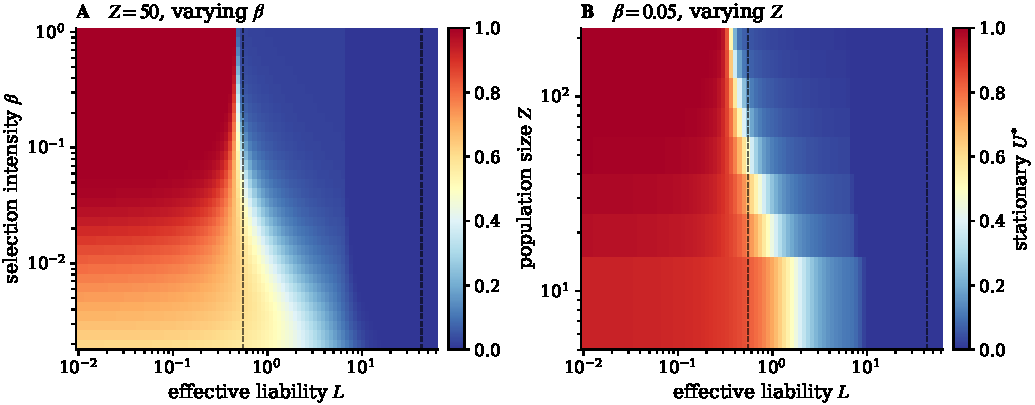
\includegraphics[width=\linewidth]{Fig7}
\caption{Stationary unsafe frequency of the finite-population pairwise
comparison process on $\{\AS,\CS,\CAS\}$ in the small-mutation limit.
\textbf{(A)} Varying selection intensity at $Z=50$. \textbf{(B)} Varying
population size at $\beta=0.05$. Dashed lines mark $L^{*}_{\CAS\to\CS}$ and
$L^{*}_{\CAS\to\AS}$.}
\label{fig:finite}
\end{figure}

\subsection{Robustness to the constants of the race}\label{sec:robust}

Every threshold in \eqref{eq:four} is a ratio of payoff differences and
therefore inherits the scale of the prize $B$ and the shape of the private
risk $p_r^{\max}$. Figure~\ref{fig:robust} recomputes them over
$B\in[10,400]$ and $p_r^{\max}\in\{0.1,0.3,0.6,0.9\}$. Three findings.

First, the liability that protects unconditional safety is a roughly constant
fraction of the prize: $L^{*}_{\CAS\to\AS}/B$ lies between $0.38$ and $0.62$
across the whole grid, decreasing weakly in $B$ and in $p_r^{\max}$. The
requirement is therefore not an artefact of the particular value $B=100$; it
says that deterring a single unsafe step in a winner-take-all race costs
around half the prize, whatever the prize is.

Second, the advantage of conditional over unconditional safety is robust and
grows with the prize: at $p_r^{\max}=0.6$ the ratio rises from $31.7$ at $B=10$
to $90.4$ at $B=400$, and over the eighteen grid points at which it is defined
it ranges from $4.4$ to $90.4$. At $p_r^{\max}=0.9$ the comparison degenerates in the
direction that strengthens the message: $L^{*}_{\CAS\to\CS}$ becomes negative,
meaning that a conditionally safe population repels $\CAS$ with \emph{no}
liability at all, while unconditional safety still requires
$L^{*}_{\CAS\to\AS}=38.4$. That $\CS$ becomes uninvadable at high private risk
also reproduces, from the selection layer, the treatment ordering reported for
the interaction layer in the source study~\citep{domingos2026falling}.

Third, the bistability window exists at every one of the $24$ grid points,
with multiplicative width between $4.19$ and $12.79$, widening in both $B$ and
$p_r^{\max}$. The liability valley is thus a structural feature of this class
of races rather than a coincidence of the baseline parameters.

We also checked the sensitivity of Corollary~\ref{cor:filter}(iii) to the
share at which the filtered design is seeded. The gap between the filtered and
unfiltered curves stays below $2.8\times10^{-3}$ for seeds up to $20\%$ at
every $L$ except $L=0.3$, where it reaches $1.2\times10^{-2}$ at a $20\%$ seed
and $0.12$ at a $35\%$ seed. The equivalence is a statement about an ecosystem
into which the filtered design enters as a minority, which is the case of
interest; it is not claimed for a population already dominated by that design.

\begin{figure}[!ht]
\centering
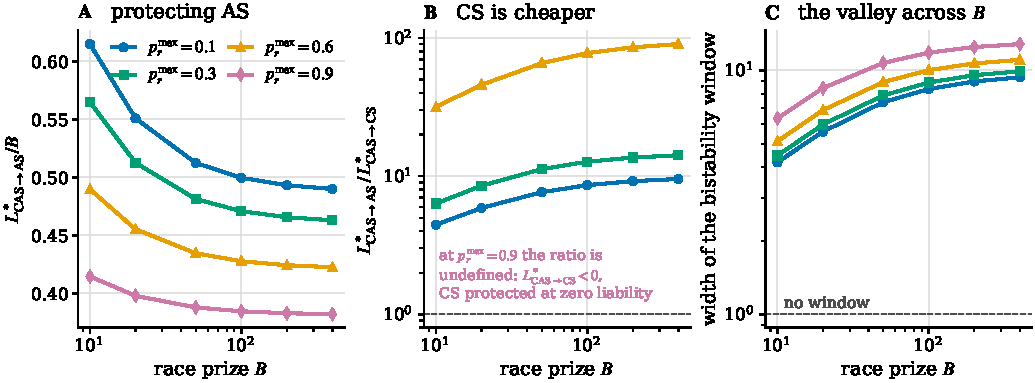
\includegraphics[width=\linewidth]{Fig8}
\caption{Thresholds across the constants of the race.
\textbf{(A)} Liability protecting unconditional safety, in units of the prize.
\textbf{(B)} Ratio $L^{*}_{\CAS\to\AS}/L^{*}_{\CAS\to\CS}$, the factor by
which unconditional safety is cheaper to invade; the $p_r^{\max}=0.9$ curve is
absent because its denominator is negative, meaning conditional safety needs
no liability at all. \textbf{(C)} Multiplicative width of the bistability
window, which is greater than one at every grid point.}
\label{fig:robust}
\end{figure}

\subsection{Execution noise and richer designs}\label{sec:noise}

The four designs are deterministic, which is what makes the matchup tables
exact and the safe face an exact twin face. Both properties are knife-edge, so
we now break them. A design is promoted to a stochastic finite-state machine
and every intended action is inverted with probability $\eta$ before it is
played and before the opponent observes it, which is the trembling-hand
perturbation of~\citet{selten1975reexamination} applied at the level of the
executed action rather than of the equilibrium concept. The joint chain over
the two
internal states is propagated exactly against the horizon law, carrying the
progress difference and the unsafe count as state and the accumulated stage
payoff as a first moment, so the evaluation remains free of sampling noise; at
$\eta=0$ it reproduces Tables~\ref{tab:payoff} and~\ref{tab:unsafe-count} to
within $1.1\times10^{-6}$, which is the horizon truncation and nothing else. We also enlarge the pool with a
generous guard $\mathsf{GCS}$ that forgives an observed unsafe action with
probability $0.25$, its aggressive counterpart $\mathsf{GCAS}$, and a
two-round punisher $\mathsf{PUN2}$ that answers one observed unsafe action
with two. The enlarged pool thus spans the severity axis along which
reciprocators divide into partners and rivals~\citep{hilbe2018partners}.

\paragraph{Noise breaks the safe face, in favour of conditional safety.}
With $\eta>0$ the twins of Proposition~\ref{prop:twins} separate, because a
conditionally safe design retaliates against its partner's trembles while an
unconditionally safe one absorbs them. The separation has a sign. A rare $\CS$
strictly invades an $\AS$ resident for every $L$ below $44.3$ at $\eta=0.01$,
$41.4$ at $0.02$, $34.4$ at $0.05$ and $26.4$ at $0.10$, and the reverse
holds above. Since the entire policy-relevant range lies below those values,
noise converts the neutrality of Theorem~\ref{thm:barrier} into a strict
gradient out of the fragile vertex. Where that gradient stops is a second
question, because the fitness difference it creates is not constant along the
face: a tremble between two copiers starts a retaliation cascade that a
tremble against an unconditionally safe partner does not, so the difference
is smaller, and taxed harder, at the conditional end than at the
unconditional one. The next proposition gives both ends, and the composition
they leave behind.

\begin{proposition}[What execution noise does to the safe face]\label{prop:rate}
Perturb the safe face so that the fitness advantage of $\CS$ over $\AS$ is
$g_{0}=\delta a_{0}-L\,\delta m_{0}$ against a pure $\AS$ resident and
$g_{1}=\delta a_{1}-L\,\delta m_{1}$ against a pure $\CS$ resident. On the
face the replicator equation is
$\dot x=x(1-x)\big[(1-x)g_{0}+xg_{1}\big]$, so neutrality breaks at first
order in the perturbation and the face is traversed in a time proportional to
the inverse of it. Under execution noise, to first order in $\eta$,
\begin{equation}
\begin{aligned}
\delta m_{0}&=\big(\mathbb{E}[T]-1\big)\,\eta=8.000\,\eta,
 &\delta a_{0}&=379.8\,\eta,\\
\delta m_{1}&=46.00\,\eta,
 &\delta a_{1}&=287.1\,\eta,
\end{aligned}
\label{eq:rate}
\end{equation}
each with an $O(\eta^{2})$ remainder. Hence
\begin{enumerate}
\item[(i)] a rare $\CS$ invades an $\AS$ resident exactly for
$L<379.8/8.000=47.5$, and a rare $\AS$ invades a $\CS$ resident exactly for
$L>287.1/46.00=6.24$;
\item[(ii)] for $L<6.24$ conditional safety sweeps the face, and the crossing
time from $x_{0}=0.05$ to $1-x_{0}$ is $\Theta(1/\eta)$: $17.8$ time units at
$\eta=10^{-3}$ and $1.78$ at $\eta=10^{-2}$, at $L=0$;
\item[(iii)] for $6.24<L<47.5$ the face carries instead a stable interior
composition, at a conditional share that is independent of $\eta$ at leading
order,
\begin{equation}
\hat x(L)=\frac{\delta a_{0}-L\,\delta m_{0}}
               {(\delta a_{0}-\delta a_{1})-L\,(\delta m_{0}-\delta m_{1})}
         =\frac{379.8-8L}{92.7+38L};
\label{eq:xhat}
\end{equation}
\item[(iv)] $\hat x(L)>x^{*}(L)$ at every $L\ge0$, where $x^{*}$ is the
critical share of Theorem~\ref{thm:barrier}: the composition execution noise
selects always lies on the protected side of the invasion barrier.
\end{enumerate}
\end{proposition}

\begin{proof}
The face carries no other force, so the replicator field restricted to it is
$x(1-x)$ times the fitness difference of the two residents, which is affine in
$x$ and interpolates $g_{0}$ and $g_{1}$; integrating gives the time, and (i)
to (iii) follow by solving linear inequalities, the interior rest point being
stable because $g_{0}>g_{1}$ whenever it exists. For $\delta m_{0}$ in
\eqref{eq:rate}, a copier facing an unconditionally safe partner mirrors each
of its \emph{own} trembles exactly once, in each of the $\mathbb{E}[T]-1$
rounds that follow the first, whereas the partner never answers; the larger
$\delta m_{1}$ is the same count against a partner that answers back, so a
single tremble is echoed for the remainder of the interaction. The remaining
coefficients are obtained from the exact evaluator, and all four are confirmed
to four digits by Richardson extrapolation on $\eta\in[10^{-4},10^{-3}]$. For
(iv), $x^{*}(L)=(42.765-L)/(40.134+3.778L)$ by inverting \eqref{eq:barrier},
and both denominators are positive at $L\ge0$, so the claim is the positivity
of
\begin{equation}
(379.8-8L)(40.134+3.778L)-(42.765-L)(92.7+38L)
  =7.776\,L^{2}-418.6\,L+11278.6,
\label{eq:margin}
\end{equation}
whose discriminant is $-1.756\times10^{5}<0$ and whose minimum value is
$5646$.
\end{proof}

Part (iv) is the substantive one, and it is stronger than the claim that the
drift acquires a direction. Above $L=6.24$ noise does \emph{not} carry the
face to the conditional vertex; it stops at $\hat x$, which falls from $1$
there to $0.022$ at the upper edge of the liability valley and to $0$ at
$L=47.5$. But it stops on the safe side of the barrier every time, and by a
margin that is widest inside the valley: $\hat x-x^{*}$ is $0.32$ at
$L^{\dagger}$ and $0.21$ at $L=10$, against $0.03$ at $L=30$. Recomputing
$\hat x$ and $x^{*}$ from the exact noisy tables rather than from the
first-order coefficients confirms this at $\eta=0.01$, $0.02$ and $0.05$ over
$L\in[0,40]$. In a finite population under Fermi imitation, selection
dominates drift on the face once $\beta Z\,|g|\gtrsim1$, which at the baseline
$\beta=0.05$, $Z=100$ and $L=0$ means $\eta\gtrsim5.3\times10^{-4}$ at the
unconditional end and $\eta\gtrsim7.0\times10^{-4}$ at the conditional one.
Exact twinning is therefore a knife-edge in the strict sense -- a tremble rate
of one in two thousand already replaces drift by selection -- and the paper's
neutral face should be read as the limiting case of a slow directed motion
towards a protected composition rather than as a description of an ecosystem
with no execution error at all.

\paragraph{The guard threshold is stable; the valley is not.}
Table~\ref{tab:noise} recomputes the thresholds. $L^{\dagger}$ moves by less
than $13\%$ over $\eta\in[0,0.10]$ and the bistability window survives at every
noise level examined, narrowing from a factor of $10.0$ to $2.6$ at
$\eta=0.20$. What does not survive is the non-monotonicity of \emph{harm}.
The reason is visible in the same table: the protected attractor stops being
protected, since $u(\CS,\CS)$ rises to $0.047$, $0.088$ and $0.186$ at
$\eta=0.01,0.02,0.05$ -- a single tremble triggers a retaliation cascade, so
residual harm grows faster than the noise that causes it. The gap between the
two attractors closes accordingly, and the largest increase of long-run harm
along the $L$-axis falls from $0.299$ at $\eta=0$ to $0.149$, $0.089$ and
$0.025$, vanishing at $\eta\ge0.075$ (Figure~\ref{fig:generality}A). The
liability valley is thus a feature of low-error ecosystems. That is not a
reassurance: above the critical noise level liability becomes monotone again
only because the state it was protecting has stopped being safe.

%% ---- begin inlined tab_noise.tex ----
\begin{table}[!ht]
\centering
\caption{Execution noise. Every quantity is recomputed exactly for designs that invert each intended action with probability $\eta$. $L^{\dagger}$ is the guard threshold, $L^{*}_{\CAS\to\AS}$ the liability protecting unconditional safety, and the window width their ratio; the barrier ratio is $L^{*}(0)/L^{*}(1)$ across the safe face. $u(\CS,\CS)$ is the residual harm of a conditionally safe population, which is zero only at $\eta=0$. The valley depth is the largest increase of the basin-averaged unsafe frequency along the $L$-axis; it vanishes at $\eta\ge0.075$.}
\label{tab:noise}
\begin{tabular}{rrrrrrr}
\toprule
$\eta$ & $L^{\dagger}$ & $L^{*}_{\CAS\to\AS}$ & width & barrier ratio & $u(\CS,\CS)$ & valley depth \\
\midrule
0.000 & 4.27 & 42.77 & 10.01 & 77.7 & 0.000 & 0.299 \\
0.010 & 4.21 & 39.20 & 9.31 & 63.7 & 0.047 & 0.149 \\
0.020 & 4.19 & 36.16 & 8.62 & 55.4 & 0.088 & 0.089 \\
0.050 & 4.30 & 29.30 & 6.82 & 44.4 & 0.186 & 0.025 \\
0.075 & 4.50 & 25.32 & 5.63 & 42.5 & 0.247 & 0.000 \\
0.100 & 4.75 & 22.34 & 4.70 & 44.0 & 0.294 & 0.000 \\
0.150 & 5.35 & 18.23 & 3.41 & 56.5 & 0.361 & 0.000 \\
0.200 & 6.02 & 15.59 & 2.59 & 89.8 & 0.405 & 0.000 \\
\bottomrule
\end{tabular}
\end{table}
%% ---- end inlined tab_noise.tex ----

\paragraph{The solo filter fails for a second reason.}
The strict filter of Section~\ref{sec:filter} separates $\CS$ from $\CAS$ by
the single first-round defection, $s(\CAS)-s(\CS)=0.132$. Under noise both
scores rise and the gap is roughly preserved ($0.127$, $0.119$ and $0.106$ at
$\eta=0.02,0.05,0.10$), but its \emph{location} moves: $s(\CS)$ reaches
$0.130$ at $\eta=0.075$. A filter calibrated on the deterministic model
therefore starts rejecting conditional safety once the error rate exceeds
about $7.6\%$ -- and conditional safety is the design that
Theorem~\ref{thm:barrier} identifies as the cheapest to protect. The
reciprocating probe of
Proposition~\ref{prop:probe} degrades from a much higher base: its margin is
$0.539$ at $\eta=0$ and still $0.449$, $0.349$ and $0.237$ at $\eta=0.02$,
$0.05$ and $0.10$, so even at a ten per cent error rate it retains more margin
than the solo probe has at no error at all.

The margin also fixes how much evaluation a filter has to buy, which is the
form in which the difference between the two probes is easiest to act on. An
evaluator that estimates each score from $n$ independent episodes separates
two designs whose true scores differ by $\Delta$ at the $95\%$ level once
$n>(1.386/\Delta)^{2}$, using the Bernoulli bound $\mathrm{sd}\le0.5$ on a
frequency. The reciprocating probe needs $n\ge7$ episodes at $\eta=0$ and
$n\ge16$ at $\eta=0.05$; the solo probe needs $n\ge111$ and $n\ge136$. Probing
against a counterpart that reciprocates is therefore not only more reliable
but roughly an order of magnitude cheaper for the same confidence, and the
gap widens rather than narrows as execution becomes noisier.

\paragraph{Weak dominance is a property of the pool.}
Theorem~\ref{thm:dominance} does not survive the enlarged pool, and the way it
fails is instructive. Against $\mathsf{PUN2}$, unconditional aggression earns
$15.48$ more than conditional aggression while committing one more unsafe
action, because $\AU$'s uninterrupted unsafe play wins the race outright
whereas $\CAS$, thrown out of phase by the two-round punishment, only ties.
The dominance is restored for $L\ge 15.48$. The corollary that follows is
weaker than the theorem but is the one that matters for policy: a filter that
removes $\AU$ is dynamically empty \emph{unless} the surviving pool contains a
design that punishes for longer than it is punished. Building such designs is
a more promising intervention than filtering, and it is an intervention on the
design layer that the selection layer does not undo.

\paragraph{The valley survives enrichment, and moves.}
Adding each of the three designs to $\{\AS,\CS,\CAS\}$, singly and together,
leaves a discontinuous upward jump of long-run harm in $L$ in every case. Its
depth is $0.299$ for the baseline pool, $0.344$ with the generous guard,
$0.163$ with the harsh guard, $0.181$ with the generous aggressor and $0.084$
with all three; at $\eta=0.02$ the corresponding depths are $0.089$, $0.055$,
$0.033$, $0.120$ and $0.044$. The location moves substantially -- the edge
sits at $L^{\dagger}=4.27$ in the baseline pool and between $12$ and $13$ in
the full pool -- so a regulator cannot read the dangerous range off the
reduced game. What is robust is that a dangerous range exists, and the harsh
punisher shrinks it rather than removing it.

\paragraph{A design that never forgives.}
The extreme point of the retaliation axis is a grim
trigger $\mathsf{GRIM}$~\citep{friedman1971supergames},
which answers one observed unsafe action with unsafe play for the remainder of
the interaction; it is the limit of $\mathsf{PUN}k$ as the punishment outlasts
the horizon, and it is the strongest guard this action space admits, earning
$31.88$ against $\CAS$ where $\CS$ earns $26.64$. Three things follow, and the
first is the most useful. It moves none of the thresholds this paper computes:
adding a design that is absent from the $\{\AS,\CS,\CAS\}$ submatrix leaves
$L^{\dagger}$ and $L^{*}_{\CAS\to\AS}$ exactly where they were, since both are
computed from that submatrix alone. The thresholds of this paper are
properties of a submatrix, and enlarging the pool moves basins rather than
those edges. It does of course add its own invasion conditions, and the edge
of the \emph{harm} curve is a property of the whole pool rather than of the
submatrix, which is why that edge does move once several designs are added at
once: between $12$ and $13$ in the full pool, as reported above. Second, the
basins it moves, it moves in the safe direction: the valley
depth falls from $0.299$ to $0.163$ with $\mathsf{GRIM}$ in the pool and to
$0.109$ with a two-round punisher alongside it. Third, it is the design that
execution noise damages most, because a single tremble is permanent: a
population of grim triggers is unsafe in $7.6\%$ of rounds at $\eta=0.01$ and
$28.9\%$ at $\eta=0.05$, against $4.7\%$ and $18.6\%$ for the copier. By
$\eta=0.05$ the valley in every enlarged pool has vanished, for the reason
that is by now familiar: the state that liability was protecting has stopped
being safe. Longer punishment is a better guard in a clean ecosystem and a
worse citizen in a noisy one, and the error rate decides which effect wins.
This reproduces, at the selection layer, the classical finding that noise
penalises unforgiving reciprocators and rewards generous
ones~\citep{molander1985optimal,nowak1992tit,fudenberg2012slow}, and that
costly punishment is paid for by the punisher~\citep{dreber2008winners}; what
is new here is that
the penalty is paid in liability charges levied on a principal rather than in
forgone payoff to the player.

\subsection{Non-linear liability, other dynamics, and structure}\label{sec:general}

\paragraph{Non-linear charges.}
Real liability is not linear in the number of incidents. Replace the charge by
$L\varphi(m)$ for a strictly increasing $\varphi$ with $\varphi(0)=0$,
normalised so that $\varphi(9)=9$, which fixes the charge on a design that is
unsafe throughout and makes $L$ comparable across shapes. Lemma~\ref{lem:affine}
survives verbatim with $\delta m$ replaced by $\delta\varphi$, so every
threshold is still a closed form, and the safe face is still an exact twin
face because $m$ vanishes identically on it and hence so does $\varphi(m)$.
Table~\ref{tab:charges} reports five shapes. The valley exists in all of them,
and the two ends of the range behave oppositely. A convex charge pushes the
window from a factor of $10.0$ to $42.3$, because it barely charges the single
unsafe action with which $\CAS$ exploits $\AS$ and so makes unconditional
safety enormously expensive to protect. A concave or capped charge does the
reverse: it charges the first incident heavily and saturates, which taxes
initiation more than escalation, and it narrows the window to $4.9$ and $7.1$.
A de minimis rule that charges nothing below two incidents never protects
unconditional safety at any liability -- its window is unbounded -- since the
exploiting action is exactly one incident. The shape of the charge is
therefore a policy lever in its own right, and it moves in the direction the
mechanism predicts: what shrinks the valley is a rule that is steep at the
first incident and flat thereafter.

%% ---- begin inlined tab_charges.tex ----
\begin{table}[!ht]
\centering
\caption{Non-linear liability. The charge is $L\varphi(m)$ with $\varphi$ increasing and normalised so that $\varphi(9)=9$, which fixes the charge on a design that is unsafe throughout and makes $L$ comparable across shapes. Every threshold remains a ratio of a payoff difference to a charge difference. A de minimis rule that does not charge a single incident never protects unconditional safety, so its window is unbounded.}
\label{tab:charges}
\begin{tabular}{lrrrr}
\toprule
charge shape & $L^{\dagger}$ & $L^{*}_{\CAS\to\AS}$ & width & valley depth \\
\midrule
linear, $\varphi(m)=m$ & 4.27 & 42.77 & 10.01 & 0.299 \\
convex, $\varphi\propto m^{2}$ & 9.11 & 384.89 & 42.25 & 0.114 \\
concave, $\varphi\propto\sqrt{m}$ & 2.93 & 14.26 & 4.87 & 0.455 \\
capped at $m=3$ & 2.00 & 14.26 & 7.11 & 0.417 \\
de minimis below $m=2$ & 6.32 & $\infty$ & $\infty$ & 0.207 \\
\bottomrule
\end{tabular}
\end{table}
%% ---- end inlined tab_charges.tex ----

\paragraph{Other selection dynamics.}
Proposition~\ref{prop:dynfree} covers imitative dynamics exactly and locates
the best-response bifurcation at the same threshold.
Figure~\ref{fig:generality}B confirms both and delimits them. Under the logit
dynamics the valley has depth $0.417$ at
$\beta=10$ and $0.171$ at $\beta=1$, and under best response with inertia
$0.433$, against $0.305$ for the replicator; the edge sits at $L^{\dagger}$ in
each case, the differences being in how much of the simplex each dynamics
routes into the unsafe basin. Aspiration-driven learning~\citep{posch1999aspiration}, in which nobody compares payoffs with
anybody, behaves differently: long-run harm is monotone
in $L$ but stops responding to it, settling at $0.237$ for every $L\ge4$ at an
aspiration of $55$. The failure mode is then not that the instrument backfires
but that it loses traction, which is a distinct and equally unwelcome
possibility.

\paragraph{Structured populations.}
The results above assume random matching, whereas evolutionary games on graphs
and lattices behave differently in
general~\citep{szabo2007graphs,perc2017statistical}. Under weak selection and
rare
mutation, the comparison of any two designs in a structured population is
governed by a single structure coefficient $\sigma$: $k$ is favoured over
$i$ -- in the sense that its fixation probability is the larger -- if and only
if
$\sigma\,\piP(k,k)+\piP(k,i)>\piP(i,k)+\sigma\,\piP(i,i)$, where $\sigma$
summarises the population structure, equals $1$ for a large well-mixed
population, and exceeds $1$ for structures that assort like with
like~\citep{tarnita2009strategy}. Two of our results can therefore be
carried over exactly. First, the safe face is neutral for \emph{every}
$\sigma$, because all four entries of $\piP$ on $\{\AS,\CS\}$ are equal and
the criterion reduces to an identity; neutrality is a property of the payoffs,
not of the matching. Second, the criterion is affine in $L$ for each $\sigma$
and gives
\begin{equation}
\begin{aligned}
\CAS \text{ favoured over } \AS &\iff \sigma\,(31.8+9L)<93.165-L,\\
\CAS \text{ favoured over } \CS &\iff \sigma\,(31.8+9L)<34.99-0.556\,L,
\end{aligned}
\label{eq:sigma}
\end{equation}
so the liability needed to keep conditional aggression out falls steeply with
assortment: $L>6.14$ suffices at $\sigma=1$, $L>3.14$ at $\sigma=1.5$ and
$L>1.56$ at $\sigma=2$, while for $\sigma\ge2.93$ unconditional safety is
protected with no liability at all. Against conditional safety the
corresponding numbers are $L>0.33$ at $\sigma=1$ and no liability at all for
$\sigma\ge1.10$. Assortment and liability are substitutes here, and the
substitution is strongly in favour of the conditional design. Two caveats
bound the criterion. It is exact only at weak selection, and weak-selection
rankings need not extrapolate to the selection strengths that a large charge
implies~\citep{wu2013extrapolating}. And it cannot settle the valley, because
it orders each pair of
designs and a bistable pair has no order; for that we need a route that keeps
the dynamics.

\paragraph{Assortative matching.}
The deterministic idealisation of structure supplies one. Under assortment at
level $r$~\citep{grafen1979hawk,eshel1982assortment,bergstrom2003algebra} a design meets a copy of
itself with probability $r$ and a partner drawn at random otherwise, so its
fitness is $r\,\piP(i,i)+(1-r)\sum_j x_j\,\piP(i,j)$, which is the replicator
dynamics of the transformed matrix
\begin{equation}
\tilde\pi(i,j)=r\,\piP(i,i)+(1-r)\,\piP(i,j).
\label{eq:assort}
\end{equation}
The transform is linear and acts on $a$ and $m$ separately, so $\tilde\pi$ is
still affine in $L$ and every closed form of this paper survives with the
assorted constants. Three consequences follow, and the first two are exact.

First, the safe face is an exact twin face at every $r$: the assortment
correction is a self-interaction term, and $\AS$ and $\CS$ are self-identical,
earning $59$ and causing no harm against themselves exactly as against each
other. Neutrality of the face is therefore a property of the payoffs and not
of the matching, in agreement with the $\sigma$-criterion above.

Second, and for the same reason, \emph{the guard threshold does not move at
all}. The comparison behind $L^{\dagger}$ is between $\CS$ and $\AS$ at a
$\CAS$-rich rest point, and the assortment correction contributes
$r\,[\piP(\CS,\CS)-\piP(\AS,\AS)]=0$ to its numerator and
$r\,[m(\CS,\CS)-m(\AS,\AS)]=0$ to its denominator, so $L^{\dagger}=4.274$ for
every $r\in[0,1]$. The lower edge of the liability valley is immune to
population structure.

Third, the upper edge is not. Writing the invasion of $\AS$ by $\CAS$ in the
assorted game gives
\begin{equation}
L^{*}_{\CAS\to\AS}(r)=\frac{42.765-74.565\,r}{1+8\,r},
\label{eq:assortupper}
\end{equation}
which falls steeply and reaches zero at $r=0.574$, beyond which unconditional
safety needs no liability at all. Because the lower edge is fixed and the
upper edge falls, the window narrows monotonically -- from a factor of $10.0$
at $r=0$ to $6.5$, $4.6$, $2.5$ and $1.4$ at $r=0.05$, $0.10$, $0.20$ and
$0.30$ -- and closes at $r=0.354$. The basin-averaged harm curves in
Figure~\ref{fig:observation}C follow: the largest increase of long-run harm
along the $L$-axis falls from $0.299$ at $r=0$ through $0.216$, $0.160$ and
$0.060$ to $0.008$ at $r=0.30$, and is exactly zero at $r=0.40$.
Table~\ref{tab:assortment} reports the sweep.

The answer to the question the $\sigma$-criterion leaves open is therefore
that network reciprocity \emph{shrinks} the liability valley, that it does so
entirely from above, and that a modest amount of it is enough: the assortment
needed to close the window is smaller than the assortment at which
unconditional safety becomes free, and much larger than the $r=0.076$ at which
conditional safety does. Structure and liability protect the two safe designs
in the opposite order, which is the same asymmetry that
Theorem~\ref{thm:barrier} reports for liability alone. We state the limits of
this: \eqref{eq:assort} is the mean-field idealisation of structure and does
not represent the local invasion geometry of a particular graph, on which
clustered aggressors can survive in regions that a well-mixed or assorted
calculation does not see.

%% ---- begin inlined tab_assortment.tex ----
\begin{table}[!ht]
\centering
\caption{Assortative matching. A design meets a copy of itself with probability $r$ and a random partner otherwise, which is the replicator dynamics of the transformed matrix $\tilde\pi(i,j)=r\,\piP(i,i)+(1-r)\,\piP(i,j)$. The guard threshold does not move at all: the assortment correction is a self-interaction term, and the two designs it compares are self-identical. The upper edge falls, so the window narrows from above and closes at $r=0.354$; a negative $L^{*}_{\CAS\to\CS}$ means conditional safety is protected with no liability at all, which happens from $r=0.076$.}
\label{tab:assortment}
\begin{tabular}{rrrrrr}
\toprule
$r$ & $L^{\dagger}$ & $L^{*}_{\CAS\to\AS}$ & $L^{*}_{\CAS\to\CS}$ & width & valley depth \\
\midrule
0.00 & 4.274 & 42.77 & 0.551 & 10.01 & 0.299 \\
0.05 & 4.274 & 27.88 & 0.182 & 6.52 & 0.216 \\
0.10 & 4.274 & 19.62 & -0.156 & 4.59 & 0.160 \\
0.20 & 4.274 & 10.71 & -0.757 & 2.51 & 0.060 \\
0.30 & 4.274 & 6.00 & -1.274 & 1.40 & 0.008 \\
0.40 & 4.274 & 3.08 & -1.723 & closed & 0.000 \\
\bottomrule
\end{tabular}
\end{table}
%% ---- end inlined tab_assortment.tex ----


\paragraph{Multi-player faces.}
Lemma~\ref{lem:twin} extends to $N$-player interactions in a weaker but usable
form. Let $a_{x}(s)$ be the payoff to a player using $x$ in a group whose
other $N-1$ members contain $s$ players using $j$, and let $k$ satisfy the
twin hypothesis $a_{k}(0)=a_{i}(0)$. At an interior rest point of the
$\{i,j\}$ face at frequency $p$ the residents have equal fitness, so the
growth rate of a rare $k$ is
$\sum_{s\ge1}\binom{N-1}{s}p^{s}(1-p)^{N-1-s}\big[a_{k}(s)-a_{i}(s)\big]$,
the $s=0$ term having vanished. Mixture-freeness therefore survives as a
sufficient condition: if $a_{k}(s)\ge a_{i}(s)$ for every $s\ge1$, strictly
for some $s$, then $k$ invades at every interior mixture, and symmetrically
for the reverse inequalities. For $N=2$ the sum has one term and the condition
is necessary as well, which recovers Lemma~\ref{lem:twin}.

\begin{figure}[!ht]
\centering

\includegraphics[width=\linewidth]{Fig9}
\caption{How far the mechanisms travel.
\textbf{(A)} Execution noise. The bistability window (right axis) persists at
every error rate examined, but the largest increase of long-run harm along the
$L$-axis (left axis) vanishes at $\eta\ge0.075$, because a conditionally safe
population stops being safe.
\textbf{(B)} Long-run harm under five selection dynamics on
$\{\AS,\CS,\CAS\}$. The replicator, logit and best-response dynamics all show
the valley at the same edge $L^{\dagger}$, as
Proposition~\ref{prop:dynfree} requires; aspiration-driven learning does not,
but stops responding to liability altogether.
\textbf{(C)} Long-run harm under five shapes of the liability charge, at equal
charge on a design that is unsafe throughout. Every shape has a valley; the
concave and capped shapes, which charge the first incident heavily and
saturate, have the narrowest.}
\label{fig:generality}
\end{figure}

\begin{figure}[!ht]
\centering
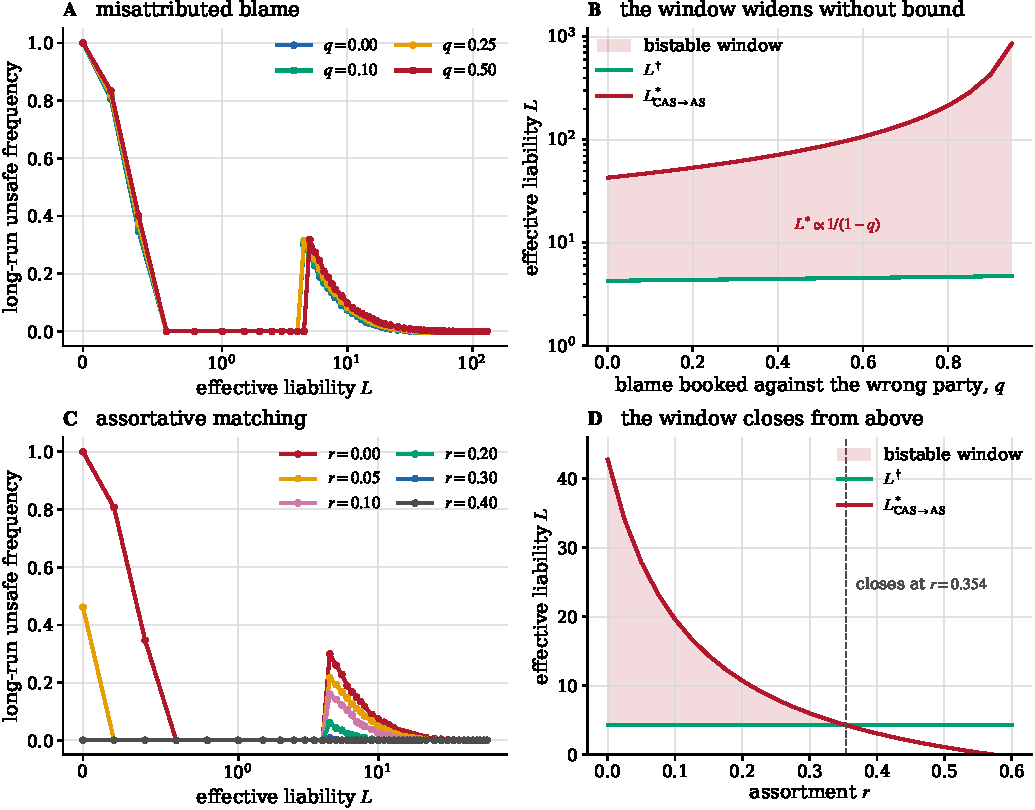
\includegraphics[width=\linewidth]{Fig10}
\caption{Two features of the environment move the valley, in opposite
directions and for the same structural reason: the lower edge of the window is
almost inert and the upper edge is not.
\textbf{(A)} Long-run harm when a fraction $q$ of the blame for an interaction
is booked against the wrong party (Section~\ref{sec:observation}).
\textbf{(B)} The two edges as functions of $q$, log scale. The guard threshold
rises by at most $11.8\%$; the liability protecting unconditional safety
diverges as $1/(1-q)$, because the design a first strike exploits has by
construction a spotless record, so blame moved onto it is blame destroyed.
\textbf{(C)} Long-run harm under assortative matching at level $r$. The
dangerous range narrows and is gone by $r=0.40$.
\textbf{(D)} The two edges as functions of $r$. Here $L^{\dagger}$ is
\emph{exactly} independent of assortment, because the assortment correction is
a self-interaction term and the two designs the threshold compares are
self-identical; the upper edge falls, so the window closes from above at
$r=0.354$.}
\label{fig:observation}
\end{figure}

\subsection{What the principal can see}\label{sec:observation}

The selection functional charges a principal for the harm its own agent
caused, which presumes that incidents are counted without error and booked
against the party that caused them. Incident data satisfy neither
presumption. We therefore replace the externality intensity by a measured one,
\begin{equation}
\hat m(i,j)=\alpha\,m(i,j)+q\,m(j,i)+c+\varepsilon_{ij},
\label{eq:channel}
\end{equation}
where $\alpha\ge0$ is the fraction of an agent's own incidents that reaches
the record, $q\ge0$ is the weight the principal places on the
\emph{counterparty's} record, $c$ is a charge levied irrespective of conduct,
and $\varepsilon$ is a zero-mean error. Three of the four terms are harmless.

\begin{proposition}[Inert measurement error]\label{prop:inertmeasure}
Let the charge be $L\hat m$ with $\hat m$ as in \eqref{eq:channel}.
\begin{enumerate}
\item[(i)] If $\mathbb{E}[\varepsilon_{ij}\mid i,j]=0$, then the replicator
field, the Nash set and every invasion threshold are exactly those of the
noiseless channel.
\item[(ii)] If $q=0$ and $\alpha=1$, the same holds for every $c$, and more
generally for every error $\hat m-m$ that depends on the counterparty alone.
\item[(iii)] If $q=0$, the channel maps each threshold $L^{*}$ to
$L^{*}/\alpha$ and leaves every ratio of thresholds unchanged.
\end{enumerate}
\end{proposition}

\begin{proof}
$\piP$ is affine in the charge base and a design meets the population rather
than any single realisation of it, so its fitness depends on the measurement
only through $\mathbb{E}\hat m$, which is (i). An error that depends on $j$
alone is a column-constant perturbation, so (ii) is
Lemma~\ref{lem:column}. For (iii) the charge is $L\alpha\,m+Lc$, whose second
term is column-constant and whose first is the baseline charge at effective
liability $L\alpha$.
\end{proof}

The content of the proposition is that variance is free, and that even bias is
free when it is bias about the counterparty rather than about the agent: a
principal may misestimate the harm of an interaction by an arbitrary amount
without disturbing a single threshold, provided the error does not depend on
which design is being charged. Part~(i) is a statement about the deterministic
objects it names, and it is exactly that: the Fermi process of
Section~\ref{sec:model} compares realised payoffs through a non-linear
imitation probability, so a zero-mean charge error does perturb its fixation
probabilities at second order even though it leaves the field, the Nash set
and the thresholds alone. Under-reporting is not free but is harmless in
a precise sense, since it only relabels the liability axis; a regime that
books one incident in three is the regime at one third of the nominal
liability, and none of the ratios in this paper move; scaling the charge by
the reciprocal of the reporting rate, the classical remedy for liability that
escapes detection~\citep{polinsky1998punitive}, restores even the labels. What
is not free is
attributing an incident to the wrong party.

\begin{proposition}[Misattribution subsidises the first strike]
\label{prop:misattr}
Set $\alpha=1-q$, $c=0$ and $\varepsilon\equiv0$ in \eqref{eq:channel}, so
that a fixed quantity of blame is split between the two parties to an
interaction and a fraction $q$ of it lands on the wrong one. Then
\begin{enumerate}
\item[(i)] the safe face remains an exact twin face for every $q$, so
Proposition~\ref{prop:twins} and Theorem~\ref{thm:barrier} apply unchanged;
\item[(ii)] $L^{*}_{\CAS\to\AS}(q)=L^{*}_{\CAS\to\AS}(0)/(1-q)$, which
diverges as $q\to1$;
\item[(iii)] $L^{\dagger}(q)=18.044/(4.222-0.444\,q)$, which rises from
$4.27$ to $4.78$ over $q\in[0,1]$, a change of at most $11.8\%$.
\end{enumerate}
The multiplicative width of the bistable window is therefore
\begin{equation}
\frac{L^{*}_{\CAS\to\AS}(q)}{L^{\dagger}(q)}
  =10.006\;\frac{1-0.1053\,q}{1-q},
\label{eq:qwindow}
\end{equation}
which is strictly increasing on $[0,1)$ and unbounded.
\end{proposition}

\begin{proof}
On $\{\AS,\CS\}$ both $m$ and its transpose vanish identically, which gives
(i). For (ii), the charge difference facing a rare $\CAS$ in an $\AS$ resident
is $(1-q)\,m(\CAS,\AS)+q\,m(\AS,\CAS)=(1-q)\cdot1+q\cdot0=1-q$, because
unconditional safety never acts unsafely against anybody; the task-payoff
difference is untouched, and the threshold is the ratio of the two. For (iii)
the same computation at a $\CAS$ resident gives
$(1-q)\,[m(\CS,\CAS)-m(\AS,\CAS)]+q\,[m(\CAS,\CS)-m(\CAS,\AS)]
 =(1-q)\,4.222+q\,3.778$, and \eqref{eq:qwindow} is the quotient.
\end{proof}

The asymmetry between (ii) and (iii) is the whole result, and it has a
one-line explanation: \emph{the design that a first strike exploits is by
construction the design with a spotless record}, so blame moved onto it is
blame destroyed, whereas the guard and the aggressor that the lower edge
compares are both active against the same opponent and lose roughly the same
amount of blame to each other. Misattribution is thus not a symmetric
degradation of the instrument. It leaves the protection of conditional safety
almost exactly where it was -- $L^{*}_{\CAS\to\CS}$ moves only from $0.551$ to
$0.623$ across the entire range of $q$ -- while making unconditional safety
progressively unprotectable, and it widens and deepens the liability valley
(Table~\ref{tab:attribution} and Figure~\ref{fig:observation}A,B). At $q=0.5$,
which is what a record that reports the interaction but not the initiator
amounts to, the dangerous range has doubled to a factor of $19.0$ of
liability.

%% ---- begin inlined tab_attribution.tex ----
\begin{table}[!ht]
\centering
\caption{Misattribution. A fixed quantity of blame is split between the two parties to an interaction and a fraction $q$ of it lands on the wrong one, so the charge base is $(1-q)\,m(i,j)+q\,m(j,i)$. The guard threshold barely moves, because both designs it compares are active against the same aggressor. The liability protecting unconditional safety diverges as $1/(1-q)$, because the design a first strike exploits has by construction a spotless record, so blame moved onto it is blame destroyed. The window widens and the valley deepens accordingly.}
\label{tab:attribution}
\begin{tabular}{rrrrrr}
\toprule
$q$ & $L^{\dagger}$ & $L^{*}_{\CAS\to\AS}$ & width & barrier ratio & valley depth \\
\midrule
0.00 & 4.27 & 42.77 & 10.01 & 77.7 & 0.299 \\
0.10 & 4.32 & 47.52 & 11.00 & 85.3 & 0.306 \\
0.25 & 4.39 & 57.02 & 12.99 & 100.6 & 0.315 \\
0.50 & 4.51 & 85.53 & 18.96 & 146.3 & 0.318 \\
\bottomrule
\end{tabular}
\end{table}
%% ---- end inlined tab_attribution.tex ----

\paragraph{Lagged enforcement.}
A principal who settles on an incident window that closed $\tau$ time units
ago charges on the composition as it was, so the fitness of design $i$ is
$\sum_j x_j(t)\,a(i,j)-L\sum_j x_j(t-\tau)\,m(i,j)$. Every rest point of the
undelayed flow is a rest point of the delayed one, because a constant history
equals the current state, and the characteristic equation of the delayed
linearisation reduces at $\lambda=0$ to that of the undelayed one, so
\emph{no invasion threshold in this paper moves under lag}. What the argument
does not exclude is an oscillatory instability at some $\tau$, which is a
different mechanism from the transversal crossings the thresholds record; we
see none in the sweeps below, but we do not rule one out. What the lag does do
is change which regime is reached. Measuring time in units
where the largest fitness difference of the selection functional is one, so
that $\tau$ is comparable with the relaxation time of the flow, the share of
random starts that end at the unsafe attractor at $L=6$ rises from $0.58$ at
$\tau=0$ to $0.79$ at $\tau=20$, while at $L=10$ it falls from $0.54$ to
$0.29$. The effect is a reallocation of basins of up to about twenty
percentage points, in a direction that depends on where in the window the
liability sits, and it does not accumulate into a change of regime.

\subsection{An eco-evolutionary ratchet}\label{sec:ratchet}

Deployed capability does not disappear. Once model weights are released they
cannot be withdrawn, and the resulting irreversibility is the feature that
distinguishes open release from every other deployment
decision~\citep{seger2023opensourcing,kapoor2024societal}. We couple the
deployment dynamics to a
state $z\in[0,1]$ measuring the stock of diffused unsafe capability, which
enters through enforcement: as a capability proliferates, attributing harm to
a particular principal becomes harder, so the liability that actually reaches
a principal decays. The coupled system is
\begin{equation}
\dot{x}=\mathrm{Rep}\big(x;\,a-L_{\mathrm{eff}}(L,z)\,m\big),
\qquad
\dot{z}=\varepsilon\,U(x)\,(1-z),
\label{eq:coupled}
\end{equation}
with $\varepsilon\ll 1$ separating the time scales. The construction differs
from reversible game--environment models~\citep{weitz2016oscillating,hauert2019asymmetric,tilman2020feedbacks} in that
$\dot z\ge 0$ identically: the environmental state is a ratchet.

We do not assume a functional form for the erosion. An \emph{erosion channel}
is any $L_{\mathrm{eff}}:\R_{\ge0}\times[0,1]\to\R_{\ge0}$ that is continuous,
non-increasing in $z$, strictly increasing in $L$, and normalised by
$L_{\mathrm{eff}}(L,0)=L$. Write
\begin{equation}
\rho \;:=\; \frac{L_{\mathrm{eff}}(L,1)}{L}\in[0,1)
\label{eq:rho}
\end{equation}
for the fraction of enforcement that survives full diffusion; for a channel
that is homogeneous in $L$, as both examples below are, $\rho$ does not depend
on $L$.

\begin{theorem}[Hysteresis width]\label{thm:hysteresis}
Let the safe attractor have $U=0$ exactly, as in
Proposition~\ref{prop:twins}, let $L_{\mathrm{eff}}$ be any erosion channel
with residual fraction $\rho$, and consider a quasi-static sweep of $L$ that
starts in the protected regime with $z=0$ at a safe-face composition
$(1-x)\AS+x\CS$. Write $L^{*}(x)$ for the barrier of
Theorem~\ref{thm:barrier} at that composition. The protected regime is lost at
$L_{\downarrow}=L^{*}(x)$, after which $z\to 1$, and is recovered on the
return sweep at $L_{\uparrow}=L^{*}(x')/\rho$, where $x'$ is the composition
the safe face is re-entered at. If the two coincide, and in particular at the
conditional vertex, where $L^{*}(1)=L^{*}_{\CAS\to\CS}$, then
\begin{equation}
\frac{L_{\uparrow}}{L_{\downarrow}}=\frac{1}{\rho}
=\begin{cases}
\dfrac{1}{1-\theta}, & L_{\mathrm{eff}}=L(1-\theta z),\\[8pt]
1+\kappa, & L_{\mathrm{eff}}=L/(1+\kappa z),
\end{cases}
\label{eq:width}
\end{equation}
for every $\varepsilon>0$ and for every channel with that $\rho$.
\end{theorem}

\begin{proof}
On the protected branch $U(x)=0$, so the second equation of \eqref{eq:coupled}
gives $\dot z=0$ for every $\varepsilon$; hence $z$ stays at its initial value
$0$ and $L_{\mathrm{eff}}=L$ by the normalisation. The branch is lost exactly
when $\CAS$ can invade the resident safe face, i.e.\ at $L=L^{*}(x)$ by
Lemma~\ref{lem:affine}, \eqref{eq:invasion} and \eqref{eq:barrier}, and this
is a condition on $\piP$ alone, so by Proposition~\ref{prop:dynfree} it does
not depend on the imitation rule. Once lost, $U>0$ on the attractor, so
$\dot z>0$ until $z=1$; since $\dot z\ge0$ always, $z$ cannot return. On the
return sweep the population therefore faces $L_{\mathrm{eff}}(L,1)=\rho L$,
and recovery requires $\rho L>L^{*}(x')$. Both thresholds are conditions on
$L_{\mathrm{eff}}$ evaluated at the two endpoints $z\in\{0,1\}$; the channel
enters only through $\rho$ and $\varepsilon$ enters nowhere, since it scales
the speed of $z$ but not its limit.
\end{proof}

The non-trivial ingredient is neither the erosion channel nor the time-scale
separation. It is Proposition~\ref{prop:twins}: because the protected branch
has $U=0$ \emph{exactly}, the ratchet variable is frozen there, so the loss
threshold is the bare invasion threshold and the shape of the channel between
its endpoints is irrelevant. Everything the channel contributes is the single
number $\rho$, and two channels sharing a $\rho$ share a width, as
\eqref{eq:width} shows for $\theta=0.9$ and $\kappa=9$.

Two remarks on the composition. The width $1/\rho$ is a ratio, so it is the
same at every safe-face composition, but the two liabilities it relates are
not: a population sitting at the unconditional vertex loses protection at
$42.765$ rather than at $0.551$, and the loop is then two orders of magnitude
higher on the $L$-axis. The loop is nevertheless self-consistent once it has
been traversed, because the safe face is always re-entered through $\CS$: on
the return sweep the guard invades the unsafe attractor as soon as
$L_{\mathrm{eff}}>L^{*}_{\CS\to\CAS}$ and holds it against $\CAS$ once
$L_{\mathrm{eff}}>L^{*}_{\CAS\to\CS}$, so $x'=1$ and $L^{*}(x')=0.551$
whatever composition the sweep started from. The sweep below is therefore run
from a $\CS$-dominated safe population, $x=0.96$, which is the composition the
return branch restores and the one at which the loop is stationary under
repetition.

Figure~\ref{fig:hysteresis} confirms the prediction numerically at
$\theta=0.9$: the descending branch loses protection between $L=0.62$ and
$L=0.54$, bracketing $L^{*}(1)=L^{*}_{\CAS\to\CS}=0.551$, and the ascending
branch recovers it at $L=5.55$ against the predicted $5.51$. The loop width is
the predicted factor of ten. Table~\ref{tab:hysteresis} repeats the sweep over
both channels, two residual fractions and a factor of twenty in $\varepsilon$
on a slightly coarser grid; the observed ratio tracks $1/\rho$ in every case
and is unchanged by $\varepsilon$, as the theorem requires.

%% ---- begin inlined tab_hysteresis.tex ----
\begin{table}[!ht]
\centering
\caption{Hysteresis width across erosion channels and diffusion speeds. The quasi-static sweep starts in the protected regime with $z=0$; $L_{\downarrow}$ and $L_{\uparrow}$ are the last grid point at which protection holds on the descending branch and the first at which it is recovered on the ascending one, on a geometric grid whose spacing is a factor of $1.08$. The predicted loss threshold is $L^{*}_{\CAS\to\CS}=0.551$ throughout. Changing $\varepsilon$ by a factor of twenty leaves the loop unchanged, and the two channels agree wherever they share a residual fraction $\rho$.}
\label{tab:hysteresis}
\begin{tabular}{llrrrrr}
\toprule
channel & $\varepsilon$ & $\rho$ & $L_{\downarrow}$ & $L_{\uparrow}$ & observed & $1/\rho$ \\
\midrule
$L(1-\theta z)$, $\theta=0.9$ & 0.05 & 0.10 & 0.564 & 5.747 & 10.19 & 10.00 \\
$L(1-\theta z)$, $\theta=0.9$ & 0.01 & 0.10 & 0.522 & 5.747 & 11.01 & 10.00 \\
$L(1-\theta z)$, $\theta=0.9$ & 0.20 & 0.10 & 0.564 & 5.747 & 10.19 & 10.00 \\
$L(1-\theta z)$, $\theta=0.5$ & 0.05 & 0.50 & 0.522 & 1.132 & 2.17 & 2.00 \\
$L/(1+\kappa z)$, $\kappa=9$ & 0.05 & 0.10 & 0.609 & 5.747 & 9.43 & 10.00 \\
$L/(1+\kappa z)$, $\kappa=1$ & 0.05 & 0.50 & 0.564 & 1.132 & 2.01 & 2.00 \\
\bottomrule
\end{tabular}
\end{table}
%% ---- end inlined tab_hysteresis.tex ----

The one assumption that does bind is exactness of $U=0$. If the protected
branch carries any residual harm -- as it does under execution noise, where a
conditionally safe population retaliates against its own trembles
(Section~\ref{sec:noise}) -- then $\dot z>0$ on that branch too, and the
protected regime is not frozen but slowly creeping. The loss threshold then
depends on $\varepsilon$, since what matters is whether the sweep is completed
before $z$ has accumulated. That is the honest boundary of the result: the
hysteresis width is exactly computable when safety is exact, and becomes a
race between the sweep and the ratchet when it is not.

\begin{figure}[!ht]
\centering
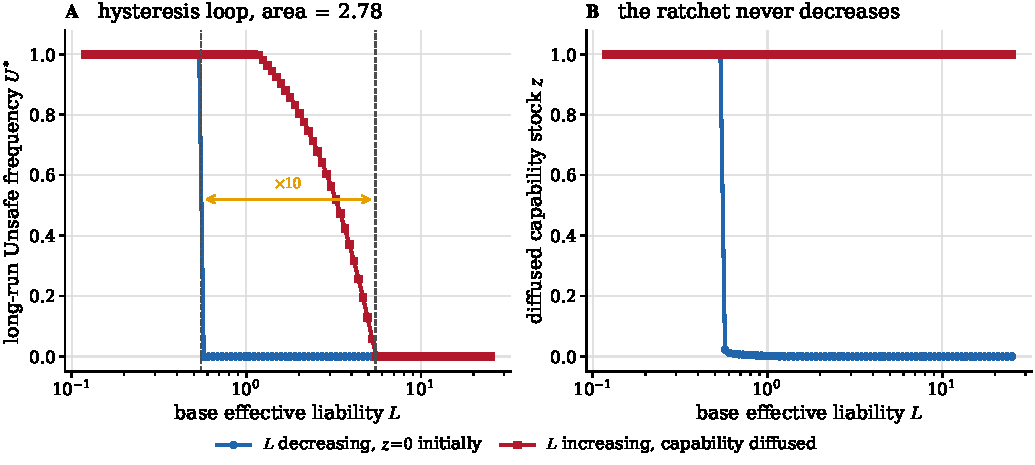
\includegraphics[width=\linewidth]{Fig11}
\caption{Irreversible capability diffusion produces hysteresis.
\textbf{(A)} Quasi-static sweep of the base effective liability, decreasing
from a protected state and then increasing again. \textbf{(B)} The ratchet
variable, which never decreases. At $\theta=0.9$ the recovery threshold is ten
times the loss threshold, as Theorem~\ref{thm:hysteresis} predicts.}
\label{fig:hysteresis}
\end{figure}

The practical content is a timing asymmetry. Because $L_{\uparrow}$ exceeds
$L_{\downarrow}$ by $1/\rho$, the cost of preventing a transition is smaller
than the cost of reversing one by exactly the factor by which enforcement
erodes, and the required overshoot is known in closed form once $\rho$ is
estimated.

\section{Discussion}\label{sec:discussion}

\paragraph{What the model says and does not say.}
The results are statements about a specific stylised race with four
deterministic designs. They are not predictions about frontier AI systems, and
the external harm $h$ has no calibration, which is why every result is stated
on the whole $L$-axis and normalised by the prize. What does transfer is the
structure. Whenever the entity that selects a design is not the entity that
plays the game, and internalises only part of the harm, the population
dynamics is the replicator equation of the selector's functional. The four
mechanisms identified here -- dominance of conditional over unconditional
aggression, neutrality of the safe face, taxation of retaliation, and
irreversibility -- then follow from qualitative features of the payoff
structure rather than from the particular numbers. The first requires only
that a conditional design imitate the unconditional one against unsafe
opponents. The second requires only that safe designs be behaviourally
indistinguishable against safe opponents. The third, by Lemma~\ref{lem:twin},
requires only that the second hold and that retaliation be classified as
harmful by the liability rule.

\paragraph{Evaluations measure the wrong object.}
Corollary~\ref{cor:filter} says that a filter defined on solo behaviour
removes a weakly dominated design. That statement is a formal counterpart of a
known practical worry, that a model may behave acceptably when probed and
unacceptably in deployment~\citep{vanderweij2024sandbagging,hammond2025multiagent}. The mechanism here
requires no deception: $\CAS$ is not hiding anything. It is simply
conditional, and an unconditional probe cannot elicit the condition. The
corrective suggested by the model is not stricter thresholds but a different
measurement, and Proposition~\ref{prop:probe} makes it precise: probe the
design against a \emph{reciprocating} counterpart. That single change widens
the margin between conditional safety and conditional aggression from $0.132$
to $0.539$, and it survives execution noise better than the solo probe does.
Probing against a maximally hostile counterpart instead is
counterproductive, because a conditionally safe design retaliates against it
in $87\%$ of rounds and is scored as unsafe. Panel B of
Figure~\ref{fig:filter} is the underlying argument -- the two orderings
disagree on exactly one design, and it is the one that governs the
equilibrium.

Stated as a protocol for the agents this model is about, the recommendation is
short. Run the candidate against a scripted counterpart that opens safe and
thereafter mirrors the candidate's previous action; score the candidate only
on the rounds that are not preceded by an unsafe action of the counterpart;
and admit on that score rather than on behaviour against a uniformly safe
environment. The scripted counterpart needs no capability of its own, which
matters because an evaluation that required a second frontier system to play
the aggressor would not be run. Two properties make the protocol cheap. The
margin it has to resolve is four times the margin of the solo probe, so at the
same confidence it needs $n\ge7$ episodes rather than $n\ge111$, and it still
needs only $n\ge16$ at a $5\%$ execution error rate. And the probe must not be
hostile: a counterpart that opens unsafe destroys the separation, because the
design one wants to admit is the design that fights back. The tension this
creates with liability is exact rather than rhetorical. An evaluation rule that
scores retaliation as unsafe and a liability rule that charges retaliation as
harm are the same mistake made at two different layers, and
Corollary~\ref{cor:valley} is what it costs when both are made at once.

\paragraph{Do not mandate unconditional safety.}
Theorem~\ref{thm:barrier} inverts a natural intuition. Unconditional safety
looks like the strictest possible design, and it is the most fragile: it
demands the highest liability of any safe composition, by a factor of $77.7$
at the baseline and up to $90.4$ at large prizes. Conditional safety is cheap to
protect because it makes exploiting it unprofitable, and at high private risk
it needs no liability at all. Because the safe face is neutral, a policy that
fixes the composition is not self-sustaining; it must be maintained against
drift. Two of the robustness checks strengthen this conclusion rather than
qualifying it. Under execution noise the face stops being neutral and settles
at a composition that lies inside the invasion barrier at every liability
(Proposition~\ref{prop:rate}), and in a structured population conditional
safety needs no liability at all once assortment exceeds $\sigma=1.10$
(Section~\ref{sec:general}). The one regime in which unconditional safety is
selected for is high liability, which is also the regime in which it is
cheapest to protect -- the instrument and the composition it induces work
against each other at every level below that.

\paragraph{Liability has a valley, and it is wide.}
Corollary~\ref{cor:valley} is the result most likely to matter outside the
model. Liability instruments are usually assumed to be monotone: more
internalisation, less harm. Here an entire decade of $L$ is worse than the
lower end of the range, because the instrument does not distinguish unsafe
behaviour that initiates from unsafe behaviour that retaliates.
Theorem~\ref{thm:guard} locates the boundary exactly, and
Section~\ref{sec:robust} shows that a window of this kind exists across the
whole range of prizes and risk levels we examined. It also survives every
enrichment of the design pool, every imitative selection dynamics and every
shape of charge that we tested, and it closes only when execution error
exceeds about $7.5\%$ -- at which point the protected state has itself stopped
being safe (Sections~\ref{sec:noise} and~\ref{sec:general}). What moves is the
location of the window, by a factor of three between the reduced pool and the
enlarged one, so the model identifies the existence of a dangerous range and
not its address.

\paragraph{Implications for multi-agent system design.}
For an engineer or a platform operator the four results read as operational
statements. First, an admission test applied to one design at a time is
dynamically inert when the design it rejects is weakly dominated by one it
admits: the filter changes which design occupies the all-unsafe state rather
than whether that state exists, and the long-run unsafe frequency is unchanged
to within $6.2\times10^{-3}$ (Corollary~\ref{cor:filter}). Admission should be
decided instead by a paired probe against a reciprocating counterpart, a
scripted opponent with no capability of its own. Second, a population resting
on a payoff-neutral face -- here the designs that never initiate, which are
exact payoff twins -- drifts along that face at no fitness cost while its
invasion barrier moves by a factor of $77.7$, from $L^{*}=42.77$ to
$L^{*}=0.55$. Nothing observable in the interaction changes meanwhile, so
resilience has to be monitored as a composition and not as an outcome. Third,
an accountability charge tuned to intermediate strength can be worse than a
weaker one: on $L\in(4.27,42.77)$ it taxes retaliation as well as initiation,
and crossing the lower edge from below lifts the basin-averaged unsafe
frequency from $0$ to $0.32$. Fourth, once the capability behind the unsafe
option has diffused, recovering a lost safe regime needs a liability larger by
the factor $1/\rho$ than the one that would have held it, so the cheap
intervention is the early one.

\paragraph{Structured populations.}
The dynamics is well mixed, but two of the four mechanisms can be carried to
structured populations exactly. Network reciprocity generally favours
cooperative strategies by clustering them~\citep{ohtsuki2006simple,santos2006structured}, and the structure
coefficient of~\citet{tarnita2009strategy} makes that quantitative here.
Equation~\eqref{eq:sigma} shows that the safe face is neutral for every
structure, and that assortment substitutes for liability at a steep rate:
protecting unconditional safety needs $L>6.14$ at $\sigma=1$ but nothing at
all at $\sigma\ge2.93$, and protecting conditional safety needs nothing at all
already at $\sigma\ge1.10$. The weak dominance of $\CAS$ over $\AU$
(Theorem~\ref{thm:dominance}) is a pointwise payoff comparison and survives
any matching structure, though Section~\ref{sec:noise} shows it does not
survive an enlarged design pool. The valley the structure coefficient cannot
reach, because it orders each pair of designs and a bistable pair has no
order; assortative matching can, since it keeps the dynamics, and the answer
is that structure shrinks the valley. Equation~\eqref{eq:assortupper} shows
the shrinking is entirely from above: the guard threshold is exactly
independent of assortment, because the assortment correction is a
self-interaction term and the two designs the threshold compares are
self-identical, while the liability that protects unconditional safety falls
to zero at $r=0.574$. The window closes at $r=0.354$. The policy reading is
that structure and liability are substitutes with very different shapes -- an
ecosystem in which agents mostly interact with their own kind needs less
liability \emph{and} has a narrower dangerous range -- and that interoperability
mandates, which lower $r$, therefore make the choice of liability level more
consequential rather than less. What remains open is the local invasion
geometry of a specific graph, which the mean-field transform
\eqref{eq:assort} does not represent and on which clustered aggressors can
persist in regions an assorted calculation does not see.

\paragraph{Reading the liability axis.}
We do not calibrate $h$, and no responsible calibration is available: the
external harm of one unsafe development step in a real deployment race is not
a measured quantity. The axis can nevertheless be read in units of the prize,
which is the one quantity a deploying firm does know. In those units the four
thresholds of \eqref{eq:four} are $L/B=0.0012$, $0.0055$, $0.043$ and $0.428$,
and Section~\ref{sec:robust} shows that the outer one stays between $0.38$ and
$0.62$ across the whole grid of prizes and risk levels. The statement that
survives is therefore a comparative one: protecting unconditional safety costs
about half the prize per unsafe step, protecting conditional safety costs
under one per cent of it, and the dangerous range lies between roughly four
per cent and half of the prize. A regulator who can estimate what a deployment
race is worth to its participants -- a procurement contract, a market
position, a first-mover advantage -- can locate a candidate regime on that
axis without ever estimating $h$. Doing so honestly for a named instrument
requires an empirical estimate of the payoff and harm matrices of real agent
designs, which is the first of the two extensions in
Section~\ref{sec:conclusion}, not something the present model supplies.

\paragraph{Instruments that do not tax retaliation.}
Proposition~\ref{prop:inert} says that a charge indexed on the counterparty's
behaviour is column-constant and therefore dynamically free, and
Corollary~\ref{cor:valley} says that the valley exists because the actual
instrument cannot tell initiation from retaliation. Three implementable
approximations follow, in increasing order of information required. The
cheapest is to shape the charge rather than to index it: Table~\ref{tab:charges}
shows that a concave or capped schedule, which charges the first incident
heavily and saturates, narrows the window to $4.9$ from the linear $10.0$,
because saturation spares the retaliator, whose incident count is high, more
than it spares the initiator, whose count is one. Deductible-and-cap
structures in insurance have exactly this shape, which is a reason to prefer
liability that is mediated by insurers~\citep{lior2022insuring,trout2025insurance} to liability
that is assessed per
incident; that insurance reshapes rather than merely transfers the incentive
to take care is the standard reading of~\citet{shavell1982insurance}, and the
present model adds that the reshaping is what narrows the dangerous range. The
second is to condition the charge on an observable proxy for who
moved first -- an incident report that records the counterparty's prior
action, which is what an audit log of an agent interaction already contains.
The third is certification of the response rule itself rather than of the
behaviour it generates~\citep{cihon2021certification}: a design certified as
retaliation-only is charged as if column-constant, which by
Lemma~\ref{lem:column} leaves the dynamics untouched. All three are
information problems rather than legal ones, which is the useful reframing:
the obstacle to a non-distorting liability rule is that incident data does not
currently record who initiated.

Section~\ref{sec:observation} turns that reframing into a quantitative
requirement, and in doing so tells a regulator which parts of a reporting
regime are worth paying for. Precision is not one of them.
Proposition~\ref{prop:inertmeasure} says that zero-mean error in counting
incidents moves no threshold, that a flat charge per deployment moves none,
that any error depending only on the counterparty moves none, and that
systematic under-reporting merely relabels the liability axis, so a regime
that books one incident in three is the regime at one third of the nominal
liability. The one qualification is that a zero-mean error is inert for the
thresholds and the deterministic field but not for the fixation probabilities
of a finite population, which respond to the second moment of the charge as
well as to its mean. Attribution is the one thing worth paying
for: by Proposition~\ref{prop:misattr} the liability that protects
unconditional safety scales as $1/(1-q)$ in the fraction $q$ of blame booked
against the wrong party, and at $q=0.5$ -- a record that establishes an
interaction went wrong but not who started it -- the dangerous range has
doubled. The instruction to a designer of an incident-reporting standard is
therefore to spend the budget on identifying the initiator and not on
measuring severity, which inverts the usual emphasis of reporting-regime
design~\citep{dixon2024hybrid}. It is also actionable
now: existing incident repositories record what happened and how badly, but
not which party in a multi-agent interaction acted
first~\citep{mcgregor2021incident}, and the serious-incident reporting duties
of the EU AI Act are drafted around a single provider and its system rather
than around an interaction between two deployed
agents~\citep{euaiact2024,buiten2023liability}. Proposals for agent
identifiers and interaction logs are exactly the reporting infrastructure that
would record the
initiator~\citep{shavit2023practices,chan2024visibility,chan2024ids}.

One caveat belongs with the counterparty-indexed charge that
Proposition~\ref{prop:inert} recommends, and it is the reason we call it an
approximation rather than a solution. A charge that depends on the counterparty
is inert on the \emph{play} dynamics precisely because it does not depend on
what the charged agent does; but it does depend on whom the agent meets, and
in any ecosystem where partners are chosen rather than drawn, that dependence
is an incentive to choose them. A principal facing a column-constant charge
has no reason to change its design and every reason to route its agent towards
counterparties with clean records, which is a matching game our model does not
contain and which would erode the very assortment
Section~\ref{sec:general} shows to be protective. The inertness result should
therefore be read as a statement about one layer: counterparty indexing moves
the distortion out of the design margin and into the matching margin. Whether
that is an improvement depends on which margin the regulator can observe.

\paragraph{Limitations.}
Five are material, and Sections~\ref{sec:noise}--\ref{sec:observation} bound three
of them rather than removing them. The interaction layer has two players, so
entry of new designs is modelled only as mutation; enriching the pool leaves
every mechanism qualitatively intact except weak dominance, which fails once a
design punishes for longer than it is punished. The valley is a low-error
phenomenon, closing at execution error rates above about $7.5\%$; whether real
agent ecosystems sit below that is an empirical question we cannot answer.
The principals are homogeneous and passive: they select on $\piP$ but do not
strategise about each other, which rules out the enforcement-avoidance
behaviour a richer model would include. The ratchet channel is assumed rather
than derived; Theorem~\ref{thm:hysteresis} now isolates exactly what does not
depend on that assumption -- everything except the residual fraction $\rho$ --
but the assumption of erosion itself remains, and the freezing of the
protected branch fails under execution noise. Finally, the analysis is
deterministic in $h$ and $\lambda$, whereas real liability arrives with
probability and delay. Section~\ref{sec:observation} removes part of that
limitation and sharpens what is left of it: the probabilistic part is
harmless, since zero-mean error and systematic under-reporting are absorbed
exactly, and the delay is harmless for the thresholds though not for the
basins, but the analysis assumes the charge is levied on an incident record
whose attribution error $q$ is exogenous and known. In a real regime, $q$ is
itself chosen by parties with an interest in its value, and a model in which
principals contest attribution rather than accept it is the natural next step.
The non-linear charges of Section~\ref{sec:general} address the shape of the
schedule but not its stochasticity.

\section{Conclusion}\label{sec:conclusion}

Separating the payoff that an AI design earns from the payoff that decides
whether it is replicated changes the dynamical system, not merely its
parameters. Working through that separation in the reduced AI race yields four
results that are invisible when the two payoffs are identified. Pre-deployment
solo evaluation cannot change the equilibrium, because it removes a weakly
dominated design. The invasion barrier protecting a safe population is
controlled by a neutrally drifting composition, and falls by a factor of
$77.7$ along it. Long-run harm is non-monotone in liability, with a bistable
window that exists at every prize and risk level we examined and traps the
population for up to $4\times10^{13}$ generations. And irreversible capability
diffusion makes the loss of a protected regime cost a known factor less than
its recovery.

Each result points at the same target. Governing an ecosystem of deployed
agents by acting on the designs -- filtering them, training them, mandating
them -- addresses the layer that does not carry the selection gradient.
Acting on the functional that principals select by does carry it, but the
instrument is not monotone, and the range in which it backfires is precisely
the range in which it is strong enough to punish retaliation and too weak to
protect unconditional safety. Locating that range for a given deployment
setting seems to us more useful than arguing about whether liability should be
strengthened.

Two extensions follow directly. Estimating the payoff and harm matrices of
real agent designs empirically, rather than from a stylised race, would place
an actual deployment ecosystem on the $L$-axis. And enriching the principals
-- letting them anticipate liability, compete, or share it -- turns the
selection functional itself into a strategic object, which is the natural
second layer of the problem.

%======================================================================

\backmatter

%%  Acknowledgements are optional and this manuscript has none to make, so the
%%  \bmhead block is omitted rather than left with placeholder text in it.  To
%%  add one, restore the block below and name the people being thanked; do not
%%  leave a bracketed placeholder in a file that gets compiled and uploaded.
%%
%%  \bmhead{Acknowledgements}
%%  The authors thank ... for comments on an earlier draft.

\section*{Declarations}

\paragraph{Funding}
%%  Accurate as of submission: the work carries no external funding.  If a
%%  grant is awarded before acceptance, replace this with the funder and the
%%  grant number written out in full.
No funding was received to assist with the preparation of this manuscript.

\paragraph{Competing interests}
The authors have no competing interests to declare that are relevant to the
content of this article.

\paragraph{Ethics approval and consent to participate}
Not applicable. This is a theoretical and computational study. It involves no
new experiments on human participants or animals. The behavioural experiment
that motivates the interaction layer was conducted and reported
by~\citet{domingos2026falling}; no data from human participants were collected
or re-analysed here.

\paragraph{Consent for publication}
Not applicable.

\paragraph{Data availability}
All quantities reported in this article are produced by the code released under
Code availability below, and are also deposited there as machine-readable files
(\texttt{results/key\_numbers.json}, \texttt{results/extensions.json},
\texttt{results/round4.json}, \texttt{results/robustness\_summary.json}).
No external or third-party dataset was used.

\paragraph{Materials availability}
Not applicable.

\paragraph{Code availability}
All code that produces the tables, the figures and every numerical value quoted
in the text is public under the MIT licence at
\sloppy\url{https://github.com/trungkiet2005/deployment-layer-selection}.
Evolutionary computations use EGTtools~\citep{domingos2023egttools}. The
repository includes the test suite that pins the reported numbers.

\paragraph{Author contributions}
All three authors contributed equally to this work. Study conception and
design, model specification, analysis, code and figures were carried out
jointly by Trung-Kiet Huynh, Dao Sy Duy Minh and Chi-Nguyen Tran. All three authors wrote,
read and approved the final manuscript.

\paragraph{Use of large language models}
%%  Springer requires generative use of an LLM to be documented; AI-assisted
%%  copy editing alone would not need declaring, but the use here went beyond
%%  copy editing, so it is declared.
Large language model assistance was used for code review, for drafting and
editing prose, and for checking bibliographic metadata against Crossref. No
text, result or reference was accepted without author verification, and the
authors take full responsibility for the content of this article.

\begin{appendices}

\section{Invasion thresholds}\label{app:tables}

Table~\ref{tab:thresholds} applies Lemma~\ref{lem:affine} to every ordered
pair of designs in Tables~\ref{tab:payoff} and~\ref{tab:unsafe-count}. Each
row is the pair $(\delta a,\delta m)$ of that invasion together with the
critical effective liability $L^{*}=\delta a/\delta m$ and the side of
$L^{*}$ on which the invader grows; the four rows that organise the paper are
collected in \eqref{eq:four}.

%% ---- begin inlined tables_thresholds.tex ----
\begin{table}[htbp]
\centering
\caption{Closed-form critical effective liabilities $L^{*}=\delta a/\delta m$ for every ordered invasion at $p_r^{\max}=0.6$. The last column states when the invader has a positive growth rate.}
\label{tab:thresholds}
\begin{tabular}{llrrrl}
\toprule
Invader & Resident & $\delta a$ & $\delta m$ & $L^{*}$ & invades \\
\midrule
AS & AU & -21.800 & -9.000 & 2.422 & $L>L^*$ \\
AS & CS & 0.000 & 0.000 & -- & -- \\
AS & CAS & -18.600 & -9.000 & 2.067 & $L>L^*$ \\
AU & AS & -10.360 & 9.000 & -1.151 & $L<L^*$ \\
AU & CS & -11.640 & 9.000 & -1.293 & $L<L^*$ \\
AU & CAS & 0.000 & 0.000 & -- & -- \\
CS & AS & 0.000 & 0.000 & -- & -- \\
CS & AU & -10.600 & -1.000 & 10.600 & $L>L^*$ \\
CS & CAS & -0.556 & -4.778 & 0.116 & $L>L^*$ \\
CAS & AS & 42.765 & 1.000 & 42.765 & $L<L^*$ \\
CAS & AU & 0.000 & 0.000 & -- & -- \\
CAS & CS & 2.631 & 4.778 & 0.551 & $L<L^*$ \\
\bottomrule
\end{tabular}
\end{table}
%% ---- end inlined tables_thresholds.tex ----

\section{The other risk treatments}\label{app:treatments}

The source experiment manipulates the maximum private setback risk
$p_r^{\max}\in\{0.1,0.6,0.9\}$ in \eqref{eq:risk}. The unsafe counts $m(i,j)$
are identical across treatments, because $p_r^{\max}$ scales the realised
payoff but leaves the stage matrix \eqref{eq:stage} and hence the action paths
untouched; only $a(i,j)$ changes. Evaluating the interaction game without
liability ($L=0$) reproduces the qualitative ordering reported in the source
study~\citep{domingos2026falling}: the neutrally stable set is
$\{\AU,\CAS\}$ at $p_r^{\max}=0.1$ and $0.6$, and $\{\CS\}$ at
$p_r^{\max}=0.9$, so high private risk favours conditional safety even before
any external liability is applied. Our main analysis uses $p_r^{\max}=0.6$,
the intermediate treatment, because it is the one in which the conditional
designs are both present and neither is trivially dominant;
Section~\ref{sec:robust} reports every threshold for the other treatments.

\end{appendices}

\bibliography{refs}

\end{document}
